% Seminar: Estimatori de Volatilitate
% Statistica Piețelor Financiare

\documentclass[9pt, aspectratio=169, t]{beamer}
%=============================================================================
% PREAMBUL COMUN - Statistica Piețelor Financiare
% Prezentări academice de calitate Harvard
% Program de licență, Academia de Studii Economice din București
%
% Utilizare: \documentclass[9pt, aspectratio=169, t]{beamer}
%            %=============================================================================
% PREAMBUL COMUN - Statistica Piețelor Financiare
% Prezentări academice de calitate Harvard
% Program de licență, Academia de Studii Economice din București
%
% Utilizare: \documentclass[9pt, aspectratio=169, t]{beamer}
%            %=============================================================================
% PREAMBUL COMUN - Statistica Piețelor Financiare
% Prezentări academice de calitate Harvard
% Program de licență, Academia de Studii Economice din București
%
% Utilizare: \documentclass[9pt, aspectratio=169, t]{beamer}
%            \input{preamble}
%            \subtitle{Seminar X: Titlul Seminarului}
%            \begin{document} ...
%=============================================================================

% Asigură încadrarea conținutului pe diapozitive
\setbeamersize{text margin left=8mm, text margin right=8mm}

%=============================================================================
% CONFIGURARE TEMĂ ȘI STIL
%=============================================================================
\usetheme{default}

% Paletă de Culori
\definecolor{MainBlue}{RGB}{26, 58, 110}
\definecolor{AccentBlue}{RGB}{26, 58, 110}
\definecolor{IDAred}{RGB}{205, 0, 0}
\definecolor{DarkGray}{RGB}{51, 51, 51}
\definecolor{MediumGray}{RGB}{128, 128, 128}
\definecolor{LightGray}{RGB}{248, 248, 248}
\definecolor{VeryLightGray}{RGB}{235, 235, 235}
\definecolor{KeynoteGray}{RGB}{218, 218, 218}
\definecolor{SectionGray}{RGB}{120, 120, 120}
\definecolor{FooterGray}{RGB}{100, 100, 100}
\definecolor{Crimson}{RGB}{220, 53, 69}
\definecolor{Forest}{RGB}{46, 125, 50}
\definecolor{Amber}{RGB}{181, 133, 63}
\definecolor{Orange}{RGB}{230, 126, 34}
\definecolor{Purple}{RGB}{142, 68, 173}

% Fundal gradient (gradient Keynote exact 315°: alb la RGB 218,218,218)
\setbeamertemplate{background}{%
    \begin{tikzpicture}[remember picture, overlay]
        \shade[shading=axis, shading angle=315,
        top color=white, bottom color=KeynoteGray]
        (current page.south west) rectangle (current page.north east);
    \end{tikzpicture}%
}
% Culoare solidă de rezervă pentru compatibilitate
\setbeamercolor{background canvas}{bg=}

\setbeamercolor{palette primary}{bg=MainBlue, fg=white}
\setbeamercolor{palette secondary}{bg=MainBlue!85, fg=white}
\setbeamercolor{palette tertiary}{bg=MainBlue!70, fg=white}
\setbeamercolor{structure}{fg=MainBlue}
\setbeamercolor{title}{fg=IDAred}
\setbeamercolor{frametitle}{fg=IDAred, bg=}
\setbeamercolor{block title}{bg=MainBlue, fg=white}
\setbeamercolor{block body}{bg=VeryLightGray, fg=DarkGray}
\setbeamercolor{block title alerted}{bg=Crimson, fg=white}
\setbeamercolor{block body alerted}{bg=Crimson!8, fg=DarkGray}
\setbeamercolor{block title example}{bg=Forest, fg=white}
\setbeamercolor{block body example}{bg=Forest!8, fg=DarkGray}
\setbeamercolor{item}{fg=MainBlue}

% Font institute mai mic pentru a evita overfull hbox pe pagina de titlu
\setbeamerfont{institute}{size=\footnotesize}

% Culori subsol
\setbeamercolor{author in head/foot}{fg=FooterGray, bg=}
\setbeamercolor{title in head/foot}{fg=FooterGray, bg=}
\setbeamercolor{date in head/foot}{fg=FooterGray, bg=}
\setbeamercolor{section in head/foot}{fg=FooterGray, bg=}
\setbeamercolor{subsection in head/foot}{fg=FooterGray, bg=}

% Stiluri marcatori
\setbeamertemplate{itemize item}{\color{MainBlue}$\boxdot$}
\setbeamertemplate{itemize subitem}{\color{MainBlue}$\blacktriangleright$}
\setbeamertemplate{itemize subsubitem}{\color{MainBlue}\tiny$\bullet$}
\setbeamertemplate{itemize/enumerate body begin}{\normalsize}
\setbeamertemplate{itemize/enumerate subbody begin}{\normalsize}

% Stiluri cuprins (bullets în loc de numere)
\setbeamertemplate{section in toc}{%
    \leavevmode\leftskip=1.5em%
    \llap{\color{MainBlue}$\boxdot$\kern0.5em}%
    \inserttocsection\par%
}

% Spațiere compactă
\setlength{\leftmargini}{10pt}
\setlength{\leftmarginii}{10pt}
\makeatletter
\def\@listi{\leftmargin\leftmargini \topsep 0pt \parsep 0pt \itemsep 0pt}
\def\@listii{\leftmargin\leftmarginii \topsep 0pt \parsep 0pt \itemsep 0pt}
\makeatother

\setbeamertemplate{navigation symbols}{}

%=============================================================================
% ANTET PERSONALIZAT
%=============================================================================
\setbeamertemplate{headline}{%
    \vskip10pt%
    \hbox to \paperwidth{%
        \hskip0.5cm%
        {\small\color{FooterGray}\renewcommand{\hyperlink}[2]{##2}\insertsectionhead}%
        \hfill%
        \textcolor{FooterGray}{\small\insertframenumber}%
        \hskip0.5cm%
    }%
    \vskip4pt%
    {\color{FooterGray}\hrule height 0.4pt}%
}

%=============================================================================
% SUBSOL PERSONALIZAT
%=============================================================================
\usepackage{fontawesome5}

\setbeamertemplate{footline}{%
    {\color{FooterGray}\hrule height 0.4pt}%
    \vskip4pt%
    \hbox to \paperwidth{%
        \hskip0.5cm%
        \textcolor{FooterGray}{\small Statistica Piețelor Financiare}%
        \hfill%
        \raisebox{-0.1em}{%
            \begin{tikzpicture}[x=0.08em, y=0.08em, line width=0.4pt]
                \draw[FooterGray] (0,3) -- (1,4) -- (2,3.5) -- (3,5) -- (4,4) -- (5,6) -- (6,5.5) -- (7,4) -- (8,5) -- (9,7) -- (10,6) -- (11,5) -- (12,6.5) -- (13,8) -- (14,7) -- (15,6) -- (16,7.5) -- (17,9) -- (18,8) -- (19,7) -- (20,8.5) -- (21,10) -- (22,9) -- (23,8) -- (24,9.5);
            \end{tikzpicture}%
        }%
        \hskip0.5cm%
    }%
    \vskip6pt%
}

%=============================================================================
% PACHETE
%=============================================================================
\usepackage[utf8]{inputenc}
\usepackage[T1]{fontenc}
\usepackage{amsmath, amssymb, amsthm}
\usepackage{mathtools}
\usepackage{bm}
\usepackage{tikz}
\usetikzlibrary{arrows.meta, positioning, shapes, calc, decorations.pathreplacing, shadings}
\usepackage{booktabs}
\usepackage{multirow}
\usepackage{array}
\usepackage{graphicx}
\usepackage{hyperref}
\usepackage{colortbl}
\usepackage{listings}
\lstset{basicstyle=\ttfamily\small, breaklines=true, frame=single, backgroundcolor=\color{VeryLightGray}}
\hypersetup{colorlinks=true, linkcolor=MainBlue, urlcolor=MainBlue}
\graphicspath{{../../logos/}{../../charts/}{../../photos/}}
\hfuzz=2pt
\vfuzz=2pt

%=============================================================================
% COMANDA QUANTLET
%=============================================================================
\newcommand{\quantlet}[2]{%
    \hfill\href{#2}{%
        \raisebox{-0.15em}{
\includegraphics[height=0.7em]{ql_logo.png}}%
        \textcolor{MainBlue}{\tiny\ #1}%
    }%
}

%=============================================================================
% PAGINĂ TITLU PERSONALIZATĂ
%=============================================================================
\defbeamertemplate*{title page}{hybrid}[1][]
{
    \vspace{0.2cm}
    \begin{center}
        \href{https://www.ase.ro}{
\includegraphics[height=1.0cm]{ase_logo.png}}\hspace{0.25cm}%
        \href{https://theida.net}{
\includegraphics[height=1.0cm]{ida_logo.png}}\hspace{0.25cm}%
        \href{https://blockchain-research-center.com}{
\includegraphics[height=1.0cm]{brc_logo.png}}\hspace{0.25cm}%
        \href{https://www.ai4efin.ase.ro}{
\includegraphics[height=1.0cm]{ai4efin_logo.png}}\hspace{0.25cm}%
        \href{https://ipe.ro/new}{
\includegraphics[height=1.0cm]{acad_logo.png}}\hspace{0.25cm}%
        \href{https://www.digital-finance-msca.com}{
\includegraphics[height=1.0cm]{msca_logo.png}}%
    \end{center}

    \vspace{0.6cm}

    \begin{center}
        \begin{minipage}{0.1\textwidth}
            \centering
            \href{https://quantlet.com}{
\includegraphics[height=1.1cm]{ql_logo.png}}
        \end{minipage}%
        \begin{minipage}{0.78\textwidth}
            \centering
            {\LARGE\bfseries\usebeamercolor[fg]{title}\inserttitle}

            \vspace{0.3cm}

            {\usebeamerfont{subtitle}\usebeamercolor[fg]{title}\insertsubtitle}
        \end{minipage}%
        \begin{minipage}{0.1\textwidth}
            \centering
            \href{https://quantinar.com}{
\includegraphics[height=1.1cm]{qr_logo.png}}
        \end{minipage}
    \end{center}

    \vspace{0.6cm}

    \hspace{0.5cm}{\usebeamerfont{author}\insertauthor}

    \vspace{0.3cm}

    \hspace{0.5cm}\begin{minipage}[t]{0.9\textwidth}
        \raggedright\small\insertinstitute
    \end{minipage}
}

%=============================================================================
% MEDII PENTRU TEOREME
%=============================================================================
\theoremstyle{definition}
\setbeamertemplate{theorems}[numbered]
\newtheorem{defn}{Definiție}
\newtheorem{thm}{Teoremă}
\newtheorem{prop}{Propoziție}
\newtheorem{rmk}{Observație}

%=============================================================================
% CENTRED MINIPAGE
%=============================================================================
\newenvironment{cminipage}[1]{%
    \par\noindent\hfill\begin{minipage}{#1}\ignorespaces
}{%
    \end{minipage}\hfill\null\par
}

%=============================================================================
% COMENZI PERSONALIZATE
%=============================================================================
\newcommand{\E}{\mathbb{E}}
\newcommand{\Var}{\text{Var}}
\newcommand{\Cov}{\text{Cov}}
\newcommand{\Corr}{\text{Corr}}
\newcommand{\R}{\mathbb{R}}
\newcommand{\N}{\mathbb{N}}
\newcommand{\Z}{\mathbb{Z}}
\newcommand{\B}{\mathbf{B}}
\newcommand{\imark}{\textcolor{MainBlue}{\textbullet}}
\newcommand{\RMSE}{\text{RMSE}}
\newcommand{\MAE}{\text{MAE}}
\newcommand{\MAPE}{\text{MAPE}}
\newcommand{\correct}{\textcolor{Forest}{\checkmark}}
\newcommand{\incorrect}{\textcolor{Crimson}{\texttimes}}

%=============================================================================
% INFORMAȚII TITLU
%=============================================================================
\title[Statistica Piețelor Financiare]{Statistica Piețelor Financiare}
\author[D.T. Pele, A. Amza]{\texorpdfstring{\begin{tabular}[t]{@{}l@{}}Daniel Traian PELE \\ Antoaneta Amza\end{tabular}}{Daniel Traian PELE, Antoaneta Amza}}
\institute{Academia de Studii Economice din București\\
IDA Institute Digital Assets\\
Blockchain Research Center\\
AI4EFin Artificial Intelligence for Energy Finance\\
Academia Română, Institutul de Prognoză Economică\\
MSCA Digital Finance}
\date{}

%            \subtitle{Seminar X: Titlul Seminarului}
%            \begin{document} ...
%=============================================================================

% Asigură încadrarea conținutului pe diapozitive
\setbeamersize{text margin left=8mm, text margin right=8mm}

%=============================================================================
% CONFIGURARE TEMĂ ȘI STIL
%=============================================================================
\usetheme{default}

% Paletă de Culori
\definecolor{MainBlue}{RGB}{26, 58, 110}
\definecolor{AccentBlue}{RGB}{26, 58, 110}
\definecolor{IDAred}{RGB}{205, 0, 0}
\definecolor{DarkGray}{RGB}{51, 51, 51}
\definecolor{MediumGray}{RGB}{128, 128, 128}
\definecolor{LightGray}{RGB}{248, 248, 248}
\definecolor{VeryLightGray}{RGB}{235, 235, 235}
\definecolor{KeynoteGray}{RGB}{218, 218, 218}
\definecolor{SectionGray}{RGB}{120, 120, 120}
\definecolor{FooterGray}{RGB}{100, 100, 100}
\definecolor{Crimson}{RGB}{220, 53, 69}
\definecolor{Forest}{RGB}{46, 125, 50}
\definecolor{Amber}{RGB}{181, 133, 63}
\definecolor{Orange}{RGB}{230, 126, 34}
\definecolor{Purple}{RGB}{142, 68, 173}

% Fundal gradient (gradient Keynote exact 315°: alb la RGB 218,218,218)
\setbeamertemplate{background}{%
    \begin{tikzpicture}[remember picture, overlay]
        \shade[shading=axis, shading angle=315,
        top color=white, bottom color=KeynoteGray]
        (current page.south west) rectangle (current page.north east);
    \end{tikzpicture}%
}
% Culoare solidă de rezervă pentru compatibilitate
\setbeamercolor{background canvas}{bg=}

\setbeamercolor{palette primary}{bg=MainBlue, fg=white}
\setbeamercolor{palette secondary}{bg=MainBlue!85, fg=white}
\setbeamercolor{palette tertiary}{bg=MainBlue!70, fg=white}
\setbeamercolor{structure}{fg=MainBlue}
\setbeamercolor{title}{fg=IDAred}
\setbeamercolor{frametitle}{fg=IDAred, bg=}
\setbeamercolor{block title}{bg=MainBlue, fg=white}
\setbeamercolor{block body}{bg=VeryLightGray, fg=DarkGray}
\setbeamercolor{block title alerted}{bg=Crimson, fg=white}
\setbeamercolor{block body alerted}{bg=Crimson!8, fg=DarkGray}
\setbeamercolor{block title example}{bg=Forest, fg=white}
\setbeamercolor{block body example}{bg=Forest!8, fg=DarkGray}
\setbeamercolor{item}{fg=MainBlue}

% Font institute mai mic pentru a evita overfull hbox pe pagina de titlu
\setbeamerfont{institute}{size=\footnotesize}

% Culori subsol
\setbeamercolor{author in head/foot}{fg=FooterGray, bg=}
\setbeamercolor{title in head/foot}{fg=FooterGray, bg=}
\setbeamercolor{date in head/foot}{fg=FooterGray, bg=}
\setbeamercolor{section in head/foot}{fg=FooterGray, bg=}
\setbeamercolor{subsection in head/foot}{fg=FooterGray, bg=}

% Stiluri marcatori
\setbeamertemplate{itemize item}{\color{MainBlue}$\boxdot$}
\setbeamertemplate{itemize subitem}{\color{MainBlue}$\blacktriangleright$}
\setbeamertemplate{itemize subsubitem}{\color{MainBlue}\tiny$\bullet$}
\setbeamertemplate{itemize/enumerate body begin}{\normalsize}
\setbeamertemplate{itemize/enumerate subbody begin}{\normalsize}

% Stiluri cuprins (bullets în loc de numere)
\setbeamertemplate{section in toc}{%
    \leavevmode\leftskip=1.5em%
    \llap{\color{MainBlue}$\boxdot$\kern0.5em}%
    \inserttocsection\par%
}

% Spațiere compactă
\setlength{\leftmargini}{10pt}
\setlength{\leftmarginii}{10pt}
\makeatletter
\def\@listi{\leftmargin\leftmargini \topsep 0pt \parsep 0pt \itemsep 0pt}
\def\@listii{\leftmargin\leftmarginii \topsep 0pt \parsep 0pt \itemsep 0pt}
\makeatother

\setbeamertemplate{navigation symbols}{}

%=============================================================================
% ANTET PERSONALIZAT
%=============================================================================
\setbeamertemplate{headline}{%
    \vskip10pt%
    \hbox to \paperwidth{%
        \hskip0.5cm%
        {\small\color{FooterGray}\renewcommand{\hyperlink}[2]{##2}\insertsectionhead}%
        \hfill%
        \textcolor{FooterGray}{\small\insertframenumber}%
        \hskip0.5cm%
    }%
    \vskip4pt%
    {\color{FooterGray}\hrule height 0.4pt}%
}

%=============================================================================
% SUBSOL PERSONALIZAT
%=============================================================================
\usepackage{fontawesome5}

\setbeamertemplate{footline}{%
    {\color{FooterGray}\hrule height 0.4pt}%
    \vskip4pt%
    \hbox to \paperwidth{%
        \hskip0.5cm%
        \textcolor{FooterGray}{\small Statistica Piețelor Financiare}%
        \hfill%
        \raisebox{-0.1em}{%
            \begin{tikzpicture}[x=0.08em, y=0.08em, line width=0.4pt]
                \draw[FooterGray] (0,3) -- (1,4) -- (2,3.5) -- (3,5) -- (4,4) -- (5,6) -- (6,5.5) -- (7,4) -- (8,5) -- (9,7) -- (10,6) -- (11,5) -- (12,6.5) -- (13,8) -- (14,7) -- (15,6) -- (16,7.5) -- (17,9) -- (18,8) -- (19,7) -- (20,8.5) -- (21,10) -- (22,9) -- (23,8) -- (24,9.5);
            \end{tikzpicture}%
        }%
        \hskip0.5cm%
    }%
    \vskip6pt%
}

%=============================================================================
% PACHETE
%=============================================================================
\usepackage[utf8]{inputenc}
\usepackage[T1]{fontenc}
\usepackage{amsmath, amssymb, amsthm}
\usepackage{mathtools}
\usepackage{bm}
\usepackage{tikz}
\usetikzlibrary{arrows.meta, positioning, shapes, calc, decorations.pathreplacing, shadings}
\usepackage{booktabs}
\usepackage{multirow}
\usepackage{array}
\usepackage{graphicx}
\usepackage{hyperref}
\usepackage{colortbl}
\usepackage{listings}
\lstset{basicstyle=\ttfamily\small, breaklines=true, frame=single, backgroundcolor=\color{VeryLightGray}}
\hypersetup{colorlinks=true, linkcolor=MainBlue, urlcolor=MainBlue}
\graphicspath{{../../logos/}{../../charts/}{../../photos/}}
\hfuzz=2pt
\vfuzz=2pt

%=============================================================================
% COMANDA QUANTLET
%=============================================================================
\newcommand{\quantlet}[2]{%
    \hfill\href{#2}{%
        \raisebox{-0.15em}{
\includegraphics[height=0.7em]{ql_logo.png}}%
        \textcolor{MainBlue}{\tiny\ #1}%
    }%
}

%=============================================================================
% PAGINĂ TITLU PERSONALIZATĂ
%=============================================================================
\defbeamertemplate*{title page}{hybrid}[1][]
{
    \vspace{0.2cm}
    \begin{center}
        \href{https://www.ase.ro}{
\includegraphics[height=1.0cm]{ase_logo.png}}\hspace{0.25cm}%
        \href{https://theida.net}{
\includegraphics[height=1.0cm]{ida_logo.png}}\hspace{0.25cm}%
        \href{https://blockchain-research-center.com}{
\includegraphics[height=1.0cm]{brc_logo.png}}\hspace{0.25cm}%
        \href{https://www.ai4efin.ase.ro}{
\includegraphics[height=1.0cm]{ai4efin_logo.png}}\hspace{0.25cm}%
        \href{https://ipe.ro/new}{
\includegraphics[height=1.0cm]{acad_logo.png}}\hspace{0.25cm}%
        \href{https://www.digital-finance-msca.com}{
\includegraphics[height=1.0cm]{msca_logo.png}}%
    \end{center}

    \vspace{0.6cm}

    \begin{center}
        \begin{minipage}{0.1\textwidth}
            \centering
            \href{https://quantlet.com}{
\includegraphics[height=1.1cm]{ql_logo.png}}
        \end{minipage}%
        \begin{minipage}{0.78\textwidth}
            \centering
            {\LARGE\bfseries\usebeamercolor[fg]{title}\inserttitle}

            \vspace{0.3cm}

            {\usebeamerfont{subtitle}\usebeamercolor[fg]{title}\insertsubtitle}
        \end{minipage}%
        \begin{minipage}{0.1\textwidth}
            \centering
            \href{https://quantinar.com}{
\includegraphics[height=1.1cm]{qr_logo.png}}
        \end{minipage}
    \end{center}

    \vspace{0.6cm}

    \hspace{0.5cm}{\usebeamerfont{author}\insertauthor}

    \vspace{0.3cm}

    \hspace{0.5cm}\begin{minipage}[t]{0.9\textwidth}
        \raggedright\small\insertinstitute
    \end{minipage}
}

%=============================================================================
% MEDII PENTRU TEOREME
%=============================================================================
\theoremstyle{definition}
\setbeamertemplate{theorems}[numbered]
\newtheorem{defn}{Definiție}
\newtheorem{thm}{Teoremă}
\newtheorem{prop}{Propoziție}
\newtheorem{rmk}{Observație}

%=============================================================================
% CENTRED MINIPAGE
%=============================================================================
\newenvironment{cminipage}[1]{%
    \par\noindent\hfill\begin{minipage}{#1}\ignorespaces
}{%
    \end{minipage}\hfill\null\par
}

%=============================================================================
% COMENZI PERSONALIZATE
%=============================================================================
\newcommand{\E}{\mathbb{E}}
\newcommand{\Var}{\text{Var}}
\newcommand{\Cov}{\text{Cov}}
\newcommand{\Corr}{\text{Corr}}
\newcommand{\R}{\mathbb{R}}
\newcommand{\N}{\mathbb{N}}
\newcommand{\Z}{\mathbb{Z}}
\newcommand{\B}{\mathbf{B}}
\newcommand{\imark}{\textcolor{MainBlue}{\textbullet}}
\newcommand{\RMSE}{\text{RMSE}}
\newcommand{\MAE}{\text{MAE}}
\newcommand{\MAPE}{\text{MAPE}}
\newcommand{\correct}{\textcolor{Forest}{\checkmark}}
\newcommand{\incorrect}{\textcolor{Crimson}{\texttimes}}

%=============================================================================
% INFORMAȚII TITLU
%=============================================================================
\title[Statistica Piețelor Financiare]{Statistica Piețelor Financiare}
\author[D.T. Pele, A. Amza]{\texorpdfstring{\begin{tabular}[t]{@{}l@{}}Daniel Traian PELE \\ Antoaneta Amza\end{tabular}}{Daniel Traian PELE, Antoaneta Amza}}
\institute{Academia de Studii Economice din București\\
IDA Institute Digital Assets\\
Blockchain Research Center\\
AI4EFin Artificial Intelligence for Energy Finance\\
Academia Română, Institutul de Prognoză Economică\\
MSCA Digital Finance}
\date{}

%            \subtitle{Seminar X: Titlul Seminarului}
%            \begin{document} ...
%=============================================================================

% Asigură încadrarea conținutului pe diapozitive
\setbeamersize{text margin left=8mm, text margin right=8mm}

%=============================================================================
% CONFIGURARE TEMĂ ȘI STIL
%=============================================================================
\usetheme{default}

% Paletă de Culori
\definecolor{MainBlue}{RGB}{26, 58, 110}
\definecolor{AccentBlue}{RGB}{26, 58, 110}
\definecolor{IDAred}{RGB}{205, 0, 0}
\definecolor{DarkGray}{RGB}{51, 51, 51}
\definecolor{MediumGray}{RGB}{128, 128, 128}
\definecolor{LightGray}{RGB}{248, 248, 248}
\definecolor{VeryLightGray}{RGB}{235, 235, 235}
\definecolor{KeynoteGray}{RGB}{218, 218, 218}
\definecolor{SectionGray}{RGB}{120, 120, 120}
\definecolor{FooterGray}{RGB}{100, 100, 100}
\definecolor{Crimson}{RGB}{220, 53, 69}
\definecolor{Forest}{RGB}{46, 125, 50}
\definecolor{Amber}{RGB}{181, 133, 63}
\definecolor{Orange}{RGB}{230, 126, 34}
\definecolor{Purple}{RGB}{142, 68, 173}

% Fundal gradient (gradient Keynote exact 315°: alb la RGB 218,218,218)
\setbeamertemplate{background}{%
    \begin{tikzpicture}[remember picture, overlay]
        \shade[shading=axis, shading angle=315,
        top color=white, bottom color=KeynoteGray]
        (current page.south west) rectangle (current page.north east);
    \end{tikzpicture}%
}
% Culoare solidă de rezervă pentru compatibilitate
\setbeamercolor{background canvas}{bg=}

\setbeamercolor{palette primary}{bg=MainBlue, fg=white}
\setbeamercolor{palette secondary}{bg=MainBlue!85, fg=white}
\setbeamercolor{palette tertiary}{bg=MainBlue!70, fg=white}
\setbeamercolor{structure}{fg=MainBlue}
\setbeamercolor{title}{fg=IDAred}
\setbeamercolor{frametitle}{fg=IDAred, bg=}
\setbeamercolor{block title}{bg=MainBlue, fg=white}
\setbeamercolor{block body}{bg=VeryLightGray, fg=DarkGray}
\setbeamercolor{block title alerted}{bg=Crimson, fg=white}
\setbeamercolor{block body alerted}{bg=Crimson!8, fg=DarkGray}
\setbeamercolor{block title example}{bg=Forest, fg=white}
\setbeamercolor{block body example}{bg=Forest!8, fg=DarkGray}
\setbeamercolor{item}{fg=MainBlue}

% Font institute mai mic pentru a evita overfull hbox pe pagina de titlu
\setbeamerfont{institute}{size=\footnotesize}

% Culori subsol
\setbeamercolor{author in head/foot}{fg=FooterGray, bg=}
\setbeamercolor{title in head/foot}{fg=FooterGray, bg=}
\setbeamercolor{date in head/foot}{fg=FooterGray, bg=}
\setbeamercolor{section in head/foot}{fg=FooterGray, bg=}
\setbeamercolor{subsection in head/foot}{fg=FooterGray, bg=}

% Stiluri marcatori
\setbeamertemplate{itemize item}{\color{MainBlue}$\boxdot$}
\setbeamertemplate{itemize subitem}{\color{MainBlue}$\blacktriangleright$}
\setbeamertemplate{itemize subsubitem}{\color{MainBlue}\tiny$\bullet$}
\setbeamertemplate{itemize/enumerate body begin}{\normalsize}
\setbeamertemplate{itemize/enumerate subbody begin}{\normalsize}

% Stiluri cuprins (bullets în loc de numere)
\setbeamertemplate{section in toc}{%
    \leavevmode\leftskip=1.5em%
    \llap{\color{MainBlue}$\boxdot$\kern0.5em}%
    \inserttocsection\par%
}

% Spațiere compactă
\setlength{\leftmargini}{10pt}
\setlength{\leftmarginii}{10pt}
\makeatletter
\def\@listi{\leftmargin\leftmargini \topsep 0pt \parsep 0pt \itemsep 0pt}
\def\@listii{\leftmargin\leftmarginii \topsep 0pt \parsep 0pt \itemsep 0pt}
\makeatother

\setbeamertemplate{navigation symbols}{}

%=============================================================================
% ANTET PERSONALIZAT
%=============================================================================
\setbeamertemplate{headline}{%
    \vskip10pt%
    \hbox to \paperwidth{%
        \hskip0.5cm%
        {\small\color{FooterGray}\renewcommand{\hyperlink}[2]{##2}\insertsectionhead}%
        \hfill%
        \textcolor{FooterGray}{\small\insertframenumber}%
        \hskip0.5cm%
    }%
    \vskip4pt%
    {\color{FooterGray}\hrule height 0.4pt}%
}

%=============================================================================
% SUBSOL PERSONALIZAT
%=============================================================================
\usepackage{fontawesome5}

\setbeamertemplate{footline}{%
    {\color{FooterGray}\hrule height 0.4pt}%
    \vskip4pt%
    \hbox to \paperwidth{%
        \hskip0.5cm%
        \textcolor{FooterGray}{\small Statistica Piețelor Financiare}%
        \hfill%
        \raisebox{-0.1em}{%
            \begin{tikzpicture}[x=0.08em, y=0.08em, line width=0.4pt]
                \draw[FooterGray] (0,3) -- (1,4) -- (2,3.5) -- (3,5) -- (4,4) -- (5,6) -- (6,5.5) -- (7,4) -- (8,5) -- (9,7) -- (10,6) -- (11,5) -- (12,6.5) -- (13,8) -- (14,7) -- (15,6) -- (16,7.5) -- (17,9) -- (18,8) -- (19,7) -- (20,8.5) -- (21,10) -- (22,9) -- (23,8) -- (24,9.5);
            \end{tikzpicture}%
        }%
        \hskip0.5cm%
    }%
    \vskip6pt%
}

%=============================================================================
% PACHETE
%=============================================================================
\usepackage[utf8]{inputenc}
\usepackage[T1]{fontenc}
\usepackage{amsmath, amssymb, amsthm}
\usepackage{mathtools}
\usepackage{bm}
\usepackage{tikz}
\usetikzlibrary{arrows.meta, positioning, shapes, calc, decorations.pathreplacing, shadings}
\usepackage{booktabs}
\usepackage{multirow}
\usepackage{array}
\usepackage{graphicx}
\usepackage{hyperref}
\usepackage{colortbl}
\usepackage{listings}
\lstset{basicstyle=\ttfamily\small, breaklines=true, frame=single, backgroundcolor=\color{VeryLightGray}}
\hypersetup{colorlinks=true, linkcolor=MainBlue, urlcolor=MainBlue}
\graphicspath{{../../logos/}{../../charts/}{../../photos/}}
\hfuzz=2pt
\vfuzz=2pt

%=============================================================================
% COMANDA QUANTLET
%=============================================================================
\newcommand{\quantlet}[2]{%
    \hfill\href{#2}{%
        \raisebox{-0.15em}{
\includegraphics[height=0.7em]{ql_logo.png}}%
        \textcolor{MainBlue}{\tiny\ #1}%
    }%
}

%=============================================================================
% PAGINĂ TITLU PERSONALIZATĂ
%=============================================================================
\defbeamertemplate*{title page}{hybrid}[1][]
{
    \vspace{0.2cm}
    \begin{center}
        \href{https://www.ase.ro}{
\includegraphics[height=1.0cm]{ase_logo.png}}\hspace{0.25cm}%
        \href{https://theida.net}{
\includegraphics[height=1.0cm]{ida_logo.png}}\hspace{0.25cm}%
        \href{https://blockchain-research-center.com}{
\includegraphics[height=1.0cm]{brc_logo.png}}\hspace{0.25cm}%
        \href{https://www.ai4efin.ase.ro}{
\includegraphics[height=1.0cm]{ai4efin_logo.png}}\hspace{0.25cm}%
        \href{https://ipe.ro/new}{
\includegraphics[height=1.0cm]{acad_logo.png}}\hspace{0.25cm}%
        \href{https://www.digital-finance-msca.com}{
\includegraphics[height=1.0cm]{msca_logo.png}}%
    \end{center}

    \vspace{0.6cm}

    \begin{center}
        \begin{minipage}{0.1\textwidth}
            \centering
            \href{https://quantlet.com}{
\includegraphics[height=1.1cm]{ql_logo.png}}
        \end{minipage}%
        \begin{minipage}{0.78\textwidth}
            \centering
            {\LARGE\bfseries\usebeamercolor[fg]{title}\inserttitle}

            \vspace{0.3cm}

            {\usebeamerfont{subtitle}\usebeamercolor[fg]{title}\insertsubtitle}
        \end{minipage}%
        \begin{minipage}{0.1\textwidth}
            \centering
            \href{https://quantinar.com}{
\includegraphics[height=1.1cm]{qr_logo.png}}
        \end{minipage}
    \end{center}

    \vspace{0.6cm}

    \hspace{0.5cm}{\usebeamerfont{author}\insertauthor}

    \vspace{0.3cm}

    \hspace{0.5cm}\begin{minipage}[t]{0.9\textwidth}
        \raggedright\small\insertinstitute
    \end{minipage}
}

%=============================================================================
% MEDII PENTRU TEOREME
%=============================================================================
\theoremstyle{definition}
\setbeamertemplate{theorems}[numbered]
\newtheorem{defn}{Definiție}
\newtheorem{thm}{Teoremă}
\newtheorem{prop}{Propoziție}
\newtheorem{rmk}{Observație}

%=============================================================================
% CENTRED MINIPAGE
%=============================================================================
\newenvironment{cminipage}[1]{%
    \par\noindent\hfill\begin{minipage}{#1}\ignorespaces
}{%
    \end{minipage}\hfill\null\par
}

%=============================================================================
% COMENZI PERSONALIZATE
%=============================================================================
\newcommand{\E}{\mathbb{E}}
\newcommand{\Var}{\text{Var}}
\newcommand{\Cov}{\text{Cov}}
\newcommand{\Corr}{\text{Corr}}
\newcommand{\R}{\mathbb{R}}
\newcommand{\N}{\mathbb{N}}
\newcommand{\Z}{\mathbb{Z}}
\newcommand{\B}{\mathbf{B}}
\newcommand{\imark}{\textcolor{MainBlue}{\textbullet}}
\newcommand{\RMSE}{\text{RMSE}}
\newcommand{\MAE}{\text{MAE}}
\newcommand{\MAPE}{\text{MAPE}}
\newcommand{\correct}{\textcolor{Forest}{\checkmark}}
\newcommand{\incorrect}{\textcolor{Crimson}{\texttimes}}

%=============================================================================
% INFORMAȚII TITLU
%=============================================================================
\title[Statistica Piețelor Financiare]{Statistica Piețelor Financiare}
\author[D.T. Pele, A. Amza]{\texorpdfstring{\begin{tabular}[t]{@{}l@{}}Daniel Traian PELE \\ Antoaneta Amza\end{tabular}}{Daniel Traian PELE, Antoaneta Amza}}
\institute{Academia de Studii Economice din București\\
IDA Institute Digital Assets\\
Blockchain Research Center\\
AI4EFin Artificial Intelligence for Energy Finance\\
Academia Română, Institutul de Prognoză Economică\\
MSCA Digital Finance}
\date{}

\subtitle{Seminar 5: Estimatori de Volatilitate}

\begin{document}

%=============================================================================
% PAGINA DE TITLU
%=============================================================================
{
\setbeamertemplate{headline}{}
\setbeamertemplate{footline}{}
\begin{frame}
    \titlepage
\end{frame}
}

%=============================================================================
% CUPRINS SEMINAR
%=============================================================================
\begin{frame}{Cuprins Seminar}
    \begin{cminipage}{0.95\textwidth}
    \begin{itemize}\setlength{\itemsep}{0pt}
        \item \textbf{Recapitulare Rapidă} -- Formule cheie și comparație estimatori
        \vspace{0.15cm}
        \item \textbf{Test Grilă} -- 10 întrebări cu variante de răspuns
        \vspace{0.15cm}
        \item \textbf{Întrebări Adevărat/Fals} -- 14 întrebări de evaluare conceptuală
        \vspace{0.15cm}
        \item \textbf{Exerciții de Calcul} -- 13 probleme rezolvate pas cu pas
        \vspace{0.15cm}
        \item \textbf{Exerciții Python} -- 4 exerciții de implementare și vizualizare
        \vspace{0.15cm}
        \item \textbf{Întrebări de Discuție} -- 4 scenarii și gândire critică
        \vspace{0.15cm}
        \item \textbf{Exerciții cu asistență AI} -- Gândire critică cu LLM
        \vspace{0.15cm}
        \item \textbf{Rezumat} -- Concluzii și pași următori
    \end{itemize}
    \end{cminipage}
\end{frame}

%=============================================================================
% RECAPITULARE RAPIDĂ
%=============================================================================
\section{Recapitulare Rapidă}

\begin{frame}[shrink=10]{Recapitulare din seminarul trecut}
    \begin{cminipage}{0.95\textwidth}
    \begin{block}{\faIcon{history} Ce am învățat în seminarele anterioare}
    \begin{itemize}\setlength{\itemsep}{0pt}
        \item \textbf{Randamente}: aritmetice $R_t = (P_t - P_{t-1})/P_{t-1}$ vs.\ logaritmice $r_t = \ln(P_t/P_{t-1})$
        \item \textbf{Proprietate cheie}: log-randamentele sunt \textbf{aditive} pe orizont: $r_{[0,T]} = \sum_{t=1}^T r_t$
        \item \textbf{Stationaritate}: prețurile nu sunt staționare, dar randamentele (de regulă) da
        \item \textbf{Variance drag}: un activ cu randament mediu $\mu$ și volatilitate $\sigma$ produce avere geometrică:
        \[
        \E[\text{creștere geometrică}] \approx \mu - \frac{\sigma^2}{2}
        \]
        \item Exemplu: dacă $\mu = 10\%$ și $\sigma = 40\%$, creșterea reală $\approx 10\% - 8\% = 2\%$ pe an
    \end{itemize}
    \end{block}
    \vspace{0.1cm}
    \begin{alertblock}{\faIcon{link} Legătura cu seminarul de azi}
    \begin{itemize}\setlength{\itemsep}{0pt}
        \item Azi învățăm să \textbf{estimăm} $\sigma$ cât mai precis --- cu cât estimatorul e mai bun, cu atât variance drag-ul e mai bine cuantificat
        \item Regula $\sqrt{T}$ de anualizare depinde de \textbf{ipoteza IID} --- vom testa când aceasta e violată
    \end{itemize}
    \end{alertblock}
    \end{cminipage}
\end{frame}

\begin{frame}[shrink=10]{Formule Cheie --- Volatilitatea Istorică}
    \begin{cminipage}{0.95\textwidth}
    \begin{columns}[T]
        \begin{column}{0.50\textwidth}
            \textbf{Volatilitatea istorică (Close-to-Close):}
            \begin{itemize}\setlength{\itemsep}{0pt}
                \item Abaterea standard a randamentelor:
                \[
                \sigma = \sqrt{\frac{1}{n-1}\sum_{t=1}^{n}(r_t - \bar{r})^2}
                \]
                \item $r_t = \ln(C_t / C_{t-1})$: randament logaritmic
                \item $\bar{r}$: media randamentelor
                \item Cel mai simplu estimator, dar folosește \textbf{doar prețurile de închidere}
            \end{itemize}
        \end{column}
        \begin{column}{0.46\textwidth}
            \textbf{Anualizarea volatilității:}
            \begin{itemize}\setlength{\itemsep}{0pt}
                \item Regula rădăcinii pătrate a timpului:
                \[
                \sigma_{\text{anual}} = \sigma_{\text{zilnic}} \times \sqrt{T}
                \]
                \item $T = 252$ zile de tranzacționare/an
                \item \textbf{Ipoteze:} randamente IID, distribuție normală
                \item Dacă randamentele sunt autocorelate, regula \textbf{nu mai este validă}
            \end{itemize}
        \end{column}
    \end{columns}
    \end{cminipage}
\end{frame}

\begin{frame}[shrink=10]{Formule Cheie --- Estimatori Bazați pe Intervale}
    \begin{cminipage}{0.95\textwidth}
    \begin{columns}[T]
        \begin{column}{0.48\textwidth}
            \textbf{Parkinson (1980):}
            \begin{itemize}\setlength{\itemsep}{0pt}
                \item Folosește prețurile \textbf{High} și \textbf{Low}:
                \[
                \sigma_P = \frac{1}{\sqrt{4\ln 2}}\sqrt{\frac{1}{n}\sum_{t=1}^{n}\!\left(\ln\frac{H_t}{L_t}\right)^{\!2}}
                \]
                \item Ipoteză: drift zero, tranzacționare continuă
            \end{itemize}

            \vspace{0.15cm}

            \textbf{Rogers-Satchell:}
            \begin{itemize}\setlength{\itemsep}{0pt}
                \item Permite \textbf{drift nenul}:
                \[
                \sigma_{RS}^2 = \frac{1}{n}\sum_{t=1}^{n}\!\left[u_t(u_t - c_t) + d_t(d_t - c_t)\right]
                \]
                \item $u_t = \ln(H_t/O_t)$, $d_t = \ln(L_t/O_t)$, $c_t = \ln(C_t/O_t)$
            \end{itemize}
        \end{column}
        \begin{column}{0.48\textwidth}
            \textbf{Garman-Klass (1980):}
            \begin{itemize}\setlength{\itemsep}{0pt}
                \item Folosește prețurile \textbf{OHLC}:
                \begin{multline*}
                \sigma_{GK}^2 = \frac{1}{n}\sum_{t=1}^{n}\Bigl[0.5\!\left(\ln\frac{H_t}{L_t}\right)^{\!2} \\
                - (2\ln 2 - 1)\!\left(\ln\frac{C_t}{O_t}\right)^{\!2}\Bigr]
                \end{multline*}
                \item \textbf{7,4$\times$} mai eficient decât close-to-close
            \end{itemize}

            \vspace{0.15cm}

            \textbf{Yang-Zhang (2000):}
            \begin{itemize}\setlength{\itemsep}{0pt}
                \item Combină overnight + intraday:
                \[
                \sigma_{YZ}^2 = \sigma_O^2 + k\,\sigma_C^2 + (1-k)\,\sigma_{RS}^2
                \]
                \item $k \approx 0.34$
                \item \textbf{14$\times$} mai eficient decât close-to-close
            \end{itemize}
        \end{column}
    \end{columns}
    \end{cminipage}
\end{frame}

\begin{frame}[shrink=10]{Diagrama Yang-Zhang: Componente vizuale}
    \begin{cminipage}{0.95\textwidth}
    \begin{center}
    \begin{tikzpicture}[>=Stealth, node distance=0.6cm, every node/.style={font=\small}]
        % Main YZ box
        \node[draw, rounded corners, fill=MainBlue!20, minimum width=4.5cm, minimum height=1.2cm, align=center, line width=1.2pt] (yz) {\textbf{Yang-Zhang} \\ $\sigma_{YZ}^2 = \sigma_O^2 + k\,\sigma_C^2 + (1{-}k)\,\sigma_{RS}^2$};

        % Three components
        \node[draw, rounded corners, fill=Crimson!18, minimum width=3.2cm, minimum height=1.6cm, align=center, below left=1.2cm and 0.8cm of yz] (overnight) {
            \textbf{Overnight} \\[2pt]
            $\sigma_O^2 = \Var\!\left(\ln\frac{O_t}{C_{t-1}}\right)$ \\[2pt]
            {\footnotesize Gap-uri între zile} \\
            {\footnotesize \textcolor{Crimson}{Earnings, macro events}}
        };

        \node[draw, rounded corners, fill=Amber!25, minimum width=3.2cm, minimum height=1.6cm, align=center, below=1.2cm of yz] (closeopen) {
            \textbf{Close-to-Open} \\[2pt]
            $k\,\sigma_C^2 = k\,\Var\!\left(\ln\frac{C_t}{O_t}\right)$ \\[2pt]
            {\footnotesize Variația intra-day} \\
            {\footnotesize \textcolor{Amber}{Ponderat cu $k \approx 0{,}34$}}
        };

        \node[draw, rounded corners, fill=Forest!18, minimum width=3.2cm, minimum height=1.6cm, align=center, below right=1.2cm and 0.8cm of yz] (rs) {
            \textbf{Rogers-Satchell} \\[2pt]
            $(1{-}k)\,\sigma_{RS}^2$ \\[2pt]
            {\footnotesize Range intra-day (OHLC)} \\
            {\footnotesize \textcolor{Forest}{Robust la drift}}
        };

        % Arrows
        \draw[->, thick, Crimson] (yz.south west) -- (overnight.north);
        \draw[->, thick, Amber] (yz.south) -- (closeopen.north);
        \draw[->, thick, Forest] (yz.south east) -- (rs.north);

        % Efficiency label
        \node[draw, rounded corners, fill=Purple!12, minimum width=2.8cm, align=center, right=0.6cm of yz] (eff) {
            \textbf{Eficiență:} \\
            $\sim 14\times$ CC \\
            {\footnotesize Cel mai eficient}
        };
        \draw[->, thick, Purple, dashed] (yz.east) -- (eff.west);
    \end{tikzpicture}
    \end{center}
    \vspace{0.1cm}
    \begin{alertblock}{Intuiție}
    \begin{itemize}\setlength{\itemsep}{0pt}
        \item Yang-Zhang descompune volatilitatea totală în 3 surse \textbf{independente}
        \item Pe piețe cu gap-uri mari (acțiuni): $\sigma_O^2$ domină $\Rightarrow$ YZ $>$ RS
        \item Pe piețe continue (crypto 24/7): $\sigma_O^2 \approx 0$ $\Rightarrow$ YZ $\approx$ RS
    \end{itemize}
    \end{alertblock}
    \end{cminipage}
\end{frame}

\begin{frame}[shrink=10]{Comparație Sintetică --- Estimatori de Volatilitate}
    \begin{cminipage}{0.95\textwidth}
    \begin{center}
    {\small
    \begin{tabular}{l c c c c}
    \toprule
    \textbf{Estimator} & \textbf{Date} & \textbf{Drift} & \textbf{Eficiență} & \textbf{Gap-uri} \\
    \midrule
    Istoric (C-C) & Close & -- & $1\times$ (referință) & Da \\
    Parkinson & H, L & Zero & $\sim 5\times$ & Nu \\
    Garman-Klass & O, H, L, C & Zero & $\sim 7{,}4\times$ & Nu \\
    Rogers-Satchell & O, H, L, C & Nenul & $\sim 8\times$ & Nu \\
    Yang-Zhang & O, H, L, C + overnight & Nenul & $\sim 14\times$ & Da \\
    \bottomrule
    \end{tabular}
    }
    \end{center}

    \vspace{0.2cm}

    \begin{itemize}\setlength{\itemsep}{0pt}
        \item \textbf{Eficiența} = raportul varianță close-to-close / varianță estimator (cu cât e mai mare, cu atât estimatorul are nevoie de mai puține observații)
        \item Toți estimatorii bazați pe intervale presupun \textbf{tranzacționare continuă} (fără salturi)
        \item Yang-Zhang este singurul care gestionează \textbf{gap-urile overnight}
    \end{itemize}
    \end{cminipage}
\end{frame}

\begin{frame}[shrink=10]{Vizualizare: Comparația estimatorilor pe date reale}
    \begin{cminipage}{0.95\textwidth}
    \begin{columns}[T]
    \begin{column}{0.58\textwidth}
    \begin{center}
    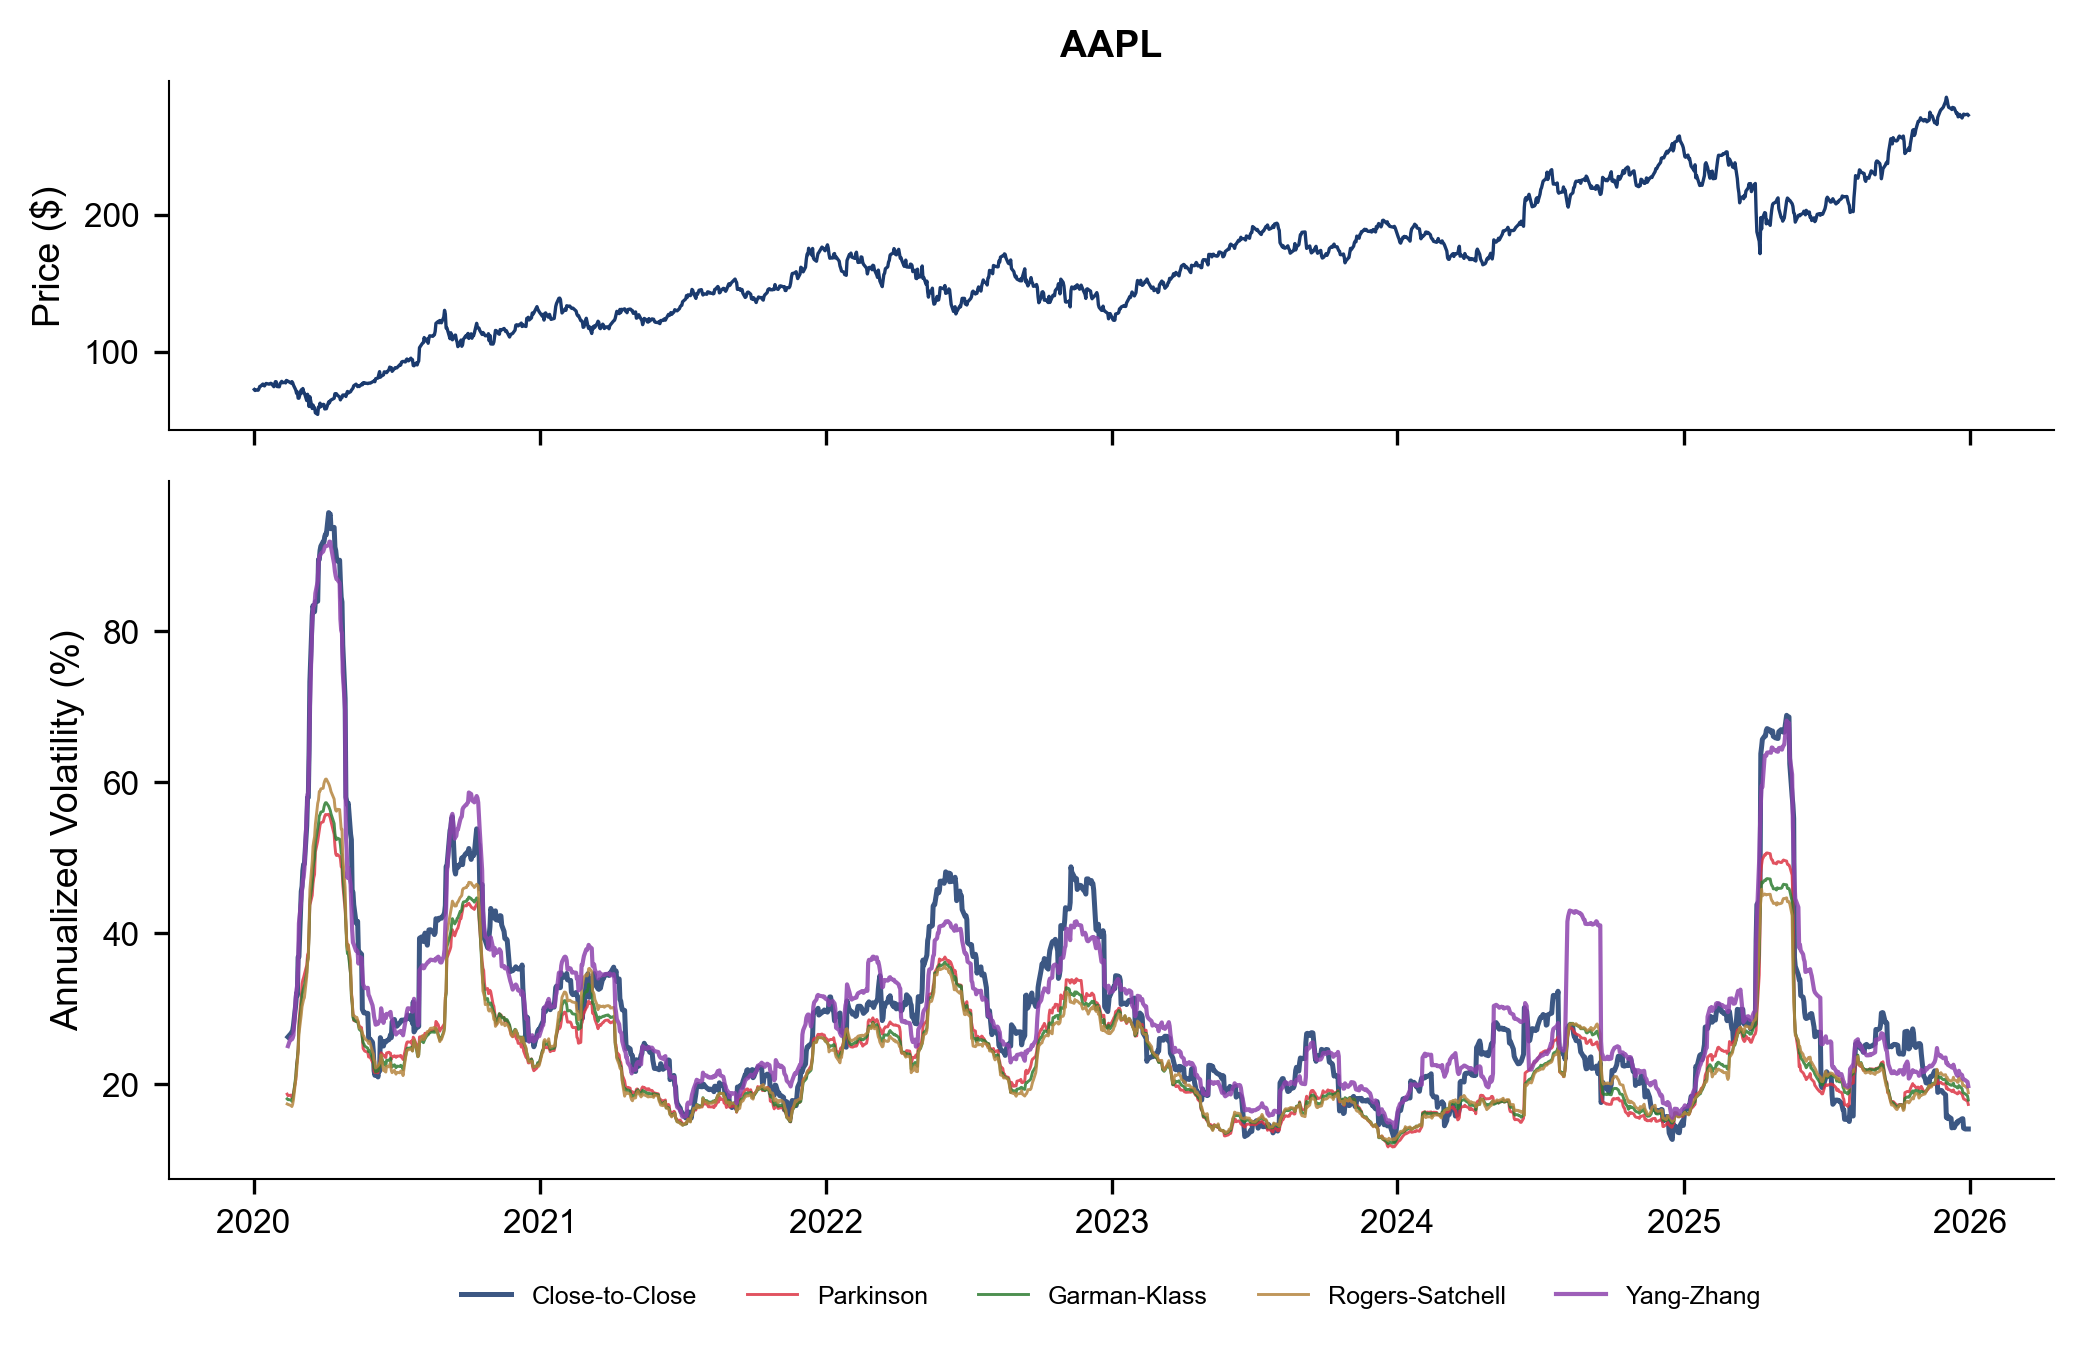
\includegraphics[width=\linewidth]{sfm_sem5_vol_rolling.png}
    \end{center}
    \end{column}
    \begin{column}{0.40\textwidth}
    \begin{exampleblock}{Observații}
    \begin{itemize}\setlength{\itemsep}{0pt}
        \item \textbf{Yang-Zhang} (violet): captează gap-urile overnight
        \item \textbf{Parkinson, GK, RS}: mai netede, ignoră gap-urile
        \item \textbf{Close-to-Close} (albastru): cel mai zgomotos
    \end{itemize}
    \end{exampleblock}
    \end{column}
    \end{columns}
    \quantlet{SFM\_ch1\_volatility\_estimators}{https://github.com/QuantLet/Stat_fin_markets/tree/master/Ch_01/SFM_ch1_volatility_estimators}
    \end{cminipage}
\end{frame}

%=============================================================================
% TEST GRILĂ
%=============================================================================
\section{Test Grilă}

\begin{frame}[shrink=10]{Test 1: Alegerea estimatorului pentru Bitcoin}
\begin{cminipage}{0.95\textwidth}
    \begin{alertblock}{Întrebare}
        Bitcoin se tranzacționează 24/7. Care estimator de volatilitate este cel mai potrivit?
    \end{alertblock}

    \vspace{0.5cm}
    \begin{block}{Variante de răspuns}
    \textcolor{MainBlue}{\textbf{(A)}} Close-to-Close (cel mai simplu)\\[3pt]
    \textcolor{MainBlue}{\textbf{(B)}} Parkinson (High-Low)\\[3pt]
    \textcolor{MainBlue}{\textbf{(C)}} Yang-Zhang (overnight)\\[3pt]
    \textcolor{MainBlue}{\textbf{(D)}} Rogers-Satchell (drift nenul)
    \end{block}
\end{cminipage}
\end{frame}

\begin{frame}[shrink=10]{Test 1: Răspuns}
\begin{cminipage}{0.95\textwidth}
    \begin{exampleblock}{Răspuns: B}
        Parkinson este cel mai potrivit pentru Bitcoin
    \end{exampleblock}

    \vspace{0.2cm}

    \begin{itemize}\setlength{\itemsep}{0pt}
        \item \textbf{Explicație:}
        \item Bitcoin se tranzacționează \textbf{24/7} --- nu există gap-uri overnight
        \item Componenta $\sigma_O^2$ din Yang-Zhang devine $\approx 0$, deci YZ $\approx$ RS --- complexitate inutilă
        \item Parkinson folosește High/Low disponibil pe orice exchange, și este $5\times$ mai eficient decât CC
        \item \textbf{Lecția contraintuitivă}: nu cel mai complex estimator e cel mai bun!
        \item Alegerea estimatorului depinde de \textbf{microstructura pieței}, nu de formulă
    \end{itemize}
\end{cminipage}
\end{frame}

\begin{frame}[shrink=10]{Test 2: Ce măsoară indicatorul Sharpe?}
\begin{cminipage}{0.95\textwidth}
    \begin{alertblock}{Întrebare}
        Ce măsoară indicatorul Sharpe (Sharpe ratio)?
    \end{alertblock}

    \vspace{0.5cm}
    \begin{block}{Variante de răspuns}
    \textcolor{MainBlue}{\textbf{(A)}} Randamentul absolut al unui activ\\[3pt]
    \textcolor{MainBlue}{\textbf{(B)}} Randamentul excesiv ajustat la risc (randament per unitate de volatilitate)\\[3pt]
    \textcolor{MainBlue}{\textbf{(C)}} Volatilitatea anualizată a randamentelor\\[3pt]
    \textcolor{MainBlue}{\textbf{(D)}} Corelația dintre activ și piață
    \end{block}
\end{cminipage}
\end{frame}

\begin{frame}[shrink=10]{Test 2: Răspuns}
\begin{cminipage}{0.95\textwidth}
    \begin{exampleblock}{Răspuns: B}
        Indicatorul Sharpe măsoară randamentul excesiv ajustat la risc: $SR = \frac{\bar{R} - R_f}{\sigma}$.
    \end{exampleblock}
    \vspace{0.2cm}
    \begin{itemize}\setlength{\itemsep}{0pt}
        \item \textbf{Explicație:}
        \item Sharpe compară cât randament \textbf{suplimentar} (peste rata fără risc $R_f$) primim pentru fiecare unitate de risc ($\sigma$)
        \item Un $SR = 1$ înseamnă că primim 1\% randament excesiv pentru fiecare 1\% volatilitate
        \item \textbf{(A)} este incorect --- randamentul absolut nu ține cont de risc
        \item \textbf{(C)} este incorect --- volatilitatea este la numitorul formulei, nu rezultatul
        \item \textbf{(D)} este incorect --- corelația cu piața este măsurată de beta ($\beta$), nu de Sharpe
    \end{itemize}
\end{cminipage}
\end{frame}

\begin{frame}[shrink=10]{Test 3: Portofoliu cu corelație perfectă negativă}
\begin{cminipage}{0.95\textwidth}
    \begin{alertblock}{Întrebare}
        Două active au aceeași volatilitate $\sigma_A = \sigma_B = \sigma$ și corelația $\rho = -1$.
        Un portofoliu echilibrat ($w_A = w_B = 0{,}5$) are volatilitatea $\sigma_p$ egală cu:
    \end{alertblock}

    \vspace{0.5cm}
    \begin{block}{Variante de răspuns}
    \textcolor{MainBlue}{\textbf{(A)}} $2\sigma$\\[3pt]
    \textcolor{MainBlue}{\textbf{(B)}} $\sigma$\\[3pt]
    \textcolor{MainBlue}{\textbf{(C)}} $0$\\[3pt]
    \textcolor{MainBlue}{\textbf{(D)}} $\sigma / \sqrt{2}$
    \end{block}
\end{cminipage}
\end{frame}

\begin{frame}[shrink=10]{Test 3: Răspuns}
\begin{cminipage}{0.95\textwidth}
    \begin{exampleblock}{Răspuns: C}
        Volatilitatea portofoliului este $\sigma_p = 0$ (hedging perfect).
    \end{exampleblock}
    \vspace{0.2cm}
    \begin{itemize}\setlength{\itemsep}{0pt}
        \item \textbf{Explicație:}
        \item $\sigma_p^2 = w_A^2 \sigma^2 + w_B^2 \sigma^2 + 2\,w_A\,w_B\,\sigma^2\,\rho$
        \item $= 0{,}25\,\sigma^2 + 0{,}25\,\sigma^2 + 2 \times 0{,}25\,\sigma^2 \times (-1) = 0{,}5\,\sigma^2 - 0{,}5\,\sigma^2 = 0$
        \item Când $\rho = -1$ și $\sigma_A = \sigma_B$, cele două active se compensează perfect
        \item \textbf{(D)} ar fi corect dacă $\rho = 0$ (active independente): $\sigma_p = \sqrt{0{,}5}\,\sigma = \sigma/\sqrt{2}$
        \item \textbf{În practică}, corelația $\rho = -1$ nu există --- este un caz-limită teoretic
    \end{itemize}
\end{cminipage}
\end{frame}

\begin{frame}[shrink=10]{Test 4: Frontiera eficientă}
\begin{cminipage}{0.95\textwidth}
    \begin{alertblock}{Întrebare}
        Frontiera eficientă (efficient frontier) reprezintă mulțimea portofoliilor care\ldots
    \end{alertblock}

    \vspace{0.5cm}
    \begin{block}{Variante de răspuns}
    \textcolor{MainBlue}{\textbf{(A)}} Minimizează randamentul pentru orice nivel de risc\\[3pt]
    \textcolor{MainBlue}{\textbf{(B)}} Maximizează indicatorul Sharpe indiferent de restricții\\[3pt]
    \textcolor{MainBlue}{\textbf{(C)}} Maximizează randamentul așteptat pentru un nivel dat de risc (sau minimizează riscul pentru un randament dat)\\[3pt]
    \textcolor{MainBlue}{\textbf{(D)}} Au risc zero prin diversificare perfectă
    \end{block}
\end{cminipage}
\end{frame}

\begin{frame}[shrink=10]{Test 4: Răspuns}
\begin{cminipage}{0.95\textwidth}
    \begin{exampleblock}{Răspuns: C}
        Frontiera eficientă conține portofoliile care maximizează randamentul așteptat pentru un nivel dat de risc, sau minimizează riscul pentru un randament dat.
    \end{exampleblock}
    \vspace{0.2cm}
    \begin{itemize}\setlength{\itemsep}{0pt}
        \item \textbf{Explicație:}
        \item Este conceptul central al teoriei portofoliului (Markowitz, 1952)
        \item \textbf{(A)} este opusul --- nimeni nu vrea să minimizeze randamentul
        \item \textbf{(B)} este parțial corect: portofoliul tangent maximizează Sharpe, dar frontiera conține \textbf{toate} portofoliile optime, nu doar unul
        \item \textbf{(D)} este imposibil --- riscul zero necesită $\rho = -1$ și ponderi specifice, nu diversificare generală
        \item Orice portofoliu \textbf{sub} frontieră este suboptimal: există un portofoliu mai bun cu același risc
    \end{itemize}
\end{cminipage}
\end{frame}

\begin{frame}[shrink=10]{Test 5: Compararea indicatorilor Sharpe}
\begin{cminipage}{0.95\textwidth}
    \begin{alertblock}{Întrebare}
        Un activ A are $SR_A = 0{,}8$ și un activ B are $SR_B = 1{,}2$.
        Pe baza randamentului ajustat la risc, care activ este mai atractiv?
    \end{alertblock}

    \vspace{0.5cm}
    \begin{block}{Variante de răspuns}
    \textcolor{MainBlue}{\textbf{(A)}} Activul A, deoarece are risc mai mic\\[3pt]
    \textcolor{MainBlue}{\textbf{(B)}} Activul B, deoarece are un Sharpe mai mare\\[3pt]
    \textcolor{MainBlue}{\textbf{(C)}} Nu putem decide fără a cunoaște corelația dintre ele\\[3pt]
    \textcolor{MainBlue}{\textbf{(D)}} Sunt echivalente ca performanță ajustată la risc
    \end{block}
\end{cminipage}
\end{frame}

\begin{frame}[shrink=10]{Test 5: Răspuns}
\begin{cminipage}{0.95\textwidth}
    \begin{exampleblock}{Răspuns: B}
        Activul B este mai atractiv pe baza randamentului ajustat la risc, deoarece $SR_B = 1{,}2 > SR_A = 0{,}8$.
    \end{exampleblock}
    \vspace{0.2cm}
    \begin{itemize}\setlength{\itemsep}{0pt}
        \item \textbf{Explicație:}
        \item Sharpe ratio este tocmai indicatorul care permite compararea activelor pe bază de randament ajustat la risc
        \item $SR_B = 1{,}2$ înseamnă 1{,}2\% randament excesiv per 1\% volatilitate --- superior lui A
        \item \textbf{(A)} nu știm dacă A are risc mai mic --- Sharpe nu ne spune $\sigma$ separat
        \item \textbf{(C)} corelația contează la construcția \textbf{portofoliului}, dar nu la compararea \textbf{individuală} a performanței
        \item \textbf{(D)} sunt diferite: B oferă cu 50\% mai mult randament per unitate de risc
        \item \textbf{Atenție}: pentru \textbf{combinarea} lor într-un portofoliu, corelația devine relevantă!
    \end{itemize}
\end{cminipage}
\end{frame}

\begin{frame}[shrink=10]{Test 6: Eficiența estimatorului Parkinson}
\begin{cminipage}{0.95\textwidth}
    \begin{alertblock}{Întrebare}
        De ce estimatorul Parkinson este mai eficient decât close-to-close?
    \end{alertblock}

    \vspace{0.5cm}
    \begin{block}{Variante de răspuns}
    \textcolor{MainBlue}{\textbf{(A)}} Folosește mai multe observații\\[3pt]
    \textcolor{MainBlue}{\textbf{(B)}} Captează informația despre mișcarea intra-zilnică prin High și Low\\[3pt]
    \textcolor{MainBlue}{\textbf{(C)}} Presupune drift nenul\\[3pt]
    \textcolor{MainBlue}{\textbf{(D)}} Include gap-urile overnight
    \end{block}
\end{cminipage}
\end{frame}

\begin{frame}[shrink=10]{Test 6: Răspuns}
\begin{cminipage}{0.95\textwidth}
    \begin{exampleblock}{Răspuns: B}
        Parkinson captează informația intra-zilnică prin prețurile High și Low.
    \end{exampleblock}
    \vspace{0.2cm}
    \begin{itemize}\setlength{\itemsep}{0pt}
        \item \textbf{Explicație:}
        \item Close-to-close folosește doar 1 punct de date pe zi (prețul de închidere)
        \item Parkinson folosește \textbf{extremele zilnice} (High, Low), care conțin informație despre \textbf{toată} traiectoria intra-zilnică
        \item Sub random walk: $\E[(\ln H/L)^2] = 4\ln 2 \cdot \sigma^2$ --- relația exactă
        \item Eficiență: $\sim 5\times$ mai eficient decât CC --- necesită $5\times$ mai puține observații
        \item \textbf{(A)} nu folosește mai multe observații, ci mai multă informație per observație
        \item \textbf{(C)} este incorect --- Parkinson presupune drift \textbf{zero}
        \item \textbf{(D)} este incorect --- doar Yang-Zhang include gap-urile overnight
    \end{itemize}
\end{cminipage}
\end{frame}

\begin{frame}[shrink=10]{Test 7: Regula $\sqrt{T}$ și autocorelația}
\begin{cminipage}{0.95\textwidth}
    \begin{alertblock}{Întrebare}
        Dacă randamentele zilnice sunt autocorelate pozitiv ($\phi > 0$), regula $\sqrt{T}$ de anualizare:
    \end{alertblock}

    \vspace{0.5cm}
    \begin{block}{Variante de răspuns}
    \textcolor{MainBlue}{\textbf{(A)}} Rămâne validă\\[3pt]
    \textcolor{MainBlue}{\textbf{(B)}} Subestimează volatilitatea anuală\\[3pt]
    \textcolor{MainBlue}{\textbf{(C)}} Supraestimează volatilitatea anuală\\[3pt]
    \textcolor{MainBlue}{\textbf{(D)}} Nu poate fi aplicată
    \end{block}
\end{cminipage}
\end{frame}

\begin{frame}[shrink=10]{Test 7: Răspuns}
\begin{cminipage}{0.95\textwidth}
    \begin{exampleblock}{Răspuns: B}
        Autocorelația pozitivă face ca regula $\sqrt{T}$ să subestimeze volatilitatea anuală.
    \end{exampleblock}
    \vspace{0.2cm}
    \begin{itemize}\setlength{\itemsep}{0pt}
        \item \textbf{Explicație:}
        \item Sub IID: $\Var(R_n) = n\sigma^2$ $\Rightarrow$ $\sigma_{\text{anual}} = \sigma_{\text{zilnic}} \times \sqrt{252}$
        \item Cu autocorelație: $\Var(R_n) \approx n\sigma^2 \cdot \frac{1+\phi}{1-\phi}$ (pentru $n$ mare)
        \item Dacă $\phi > 0$: factorul $\frac{1+\phi}{1-\phi} > 1$ $\Rightarrow$ volatilitatea reală este \textbf{mai mare}
        \item \textbf{Exemplu}: $\phi = 0{,}3$, $\sigma_{\text{zilnic}} = 1\%$:
        \begin{itemize}\setlength{\itemsep}{0pt}
            \item Regula $\sqrt{T}$: $15{,}87\%$
            \item Corect: $15{,}87\% \times \sqrt{1{,}3/0{,}7} = \mathbf{21{,}63\%}$ --- subestimare de 36\%!
        \end{itemize}
    \end{itemize}
\end{cminipage}
\end{frame}

\begin{frame}[shrink=10]{Test 8: Variance drag}
\begin{cminipage}{0.95\textwidth}
    \begin{alertblock}{Întrebare}
        Un activ crește cu 20\% într-o lună, apoi scade cu 20\% în luna următoare. Care este randamentul total?
    \end{alertblock}

    \vspace{0.5cm}
    \begin{block}{Variante de răspuns}
    \textcolor{MainBlue}{\textbf{(A)}} 0\% (se compensează perfect)\\[3pt]
    \textcolor{MainBlue}{\textbf{(B)}} $-4\%$ (pierdere netă)\\[3pt]
    \textcolor{MainBlue}{\textbf{(C)}} $+4\%$ (câștig net)\\[3pt]
    \textcolor{MainBlue}{\textbf{(D)}} Depinde de prețul inițial
    \end{block}
\end{cminipage}
\end{frame}

\begin{frame}[shrink=10]{Test 8: Răspuns}
\begin{cminipage}{0.95\textwidth}
    \begin{exampleblock}{Răspuns: B}
        $\$100 \to \$120 \to \$96$ --- pierdere de 4\% (variance drag)
    \end{exampleblock}
    \vspace{0.2cm}
    \begin{itemize}\setlength{\itemsep}{0pt}
        \item \textbf{Explicație:}
        \item $100 \times 1{,}20 \times 0{,}80 = 96$ --- pierdere de 4\%
        \item Aceasta este \textbf{variance drag}: volatilitatea erodează averea chiar dacă randamentele aritmetice se compensează
        \item Formula generală: $\E[\text{creștere geometrică}] \approx \mu - \frac{\sigma^2}{2}$
        \item Cu cât volatilitatea este mai mare, cu atât pierderea este mai mare
        \item \textbf{Exemplu BTC}: $\sigma \approx 70\%$ $\Rightarrow$ drag $= 0{,}70^2/2 = 24{,}5\%$/an --- devastator!
    \end{itemize}
\end{cminipage}
\end{frame}

\begin{frame}[shrink=10]{Test 9: Yang-Zhang pe piețe continue}
\begin{cminipage}{0.95\textwidth}
    \begin{alertblock}{Întrebare}
        Pe o piață cu tranzacționare continuă (fără gap-uri overnight), Yang-Zhang converge la:
    \end{alertblock}

    \vspace{0.5cm}
    \begin{block}{Variante de răspuns}
    \textcolor{MainBlue}{\textbf{(A)}} Close-to-Close\\[3pt]
    \textcolor{MainBlue}{\textbf{(B)}} Parkinson\\[3pt]
    \textcolor{MainBlue}{\textbf{(C)}} Rogers-Satchell\\[3pt]
    \textcolor{MainBlue}{\textbf{(D)}} Garman-Klass
    \end{block}
\end{cminipage}
\end{frame}

\begin{frame}[shrink=10]{Test 9: Răspuns}
\begin{cminipage}{0.95\textwidth}
    \begin{exampleblock}{Răspuns: C}
        Fără gap-uri overnight, Yang-Zhang converge la Rogers-Satchell.
    \end{exampleblock}
    \vspace{0.2cm}
    \begin{itemize}\setlength{\itemsep}{0pt}
        \item \textbf{Explicație:}
        \item $\sigma_{YZ}^2 = \sigma_O^2 + k\,\sigma_C^2 + (1-k)\,\sigma_{RS}^2$
        \item Fără gap-uri: $O_t = C_{t-1}$ $\Rightarrow$ $\sigma_O^2 = \Var(\ln(O_t/C_{t-1})) = 0$
        \item Formula devine: $\sigma_{YZ}^2 \approx (1-k)\,\sigma_{RS}^2 + k\,\sigma_C^2 \approx \sigma_{RS}^2$
        \item Concluzie: pe piețe 24/7 (crypto), Yang-Zhang nu aduce valoare suplimentară față de Rogers-Satchell
        \item Aceasta explică de ce CC $\approx$ YZ pe Bitcoin --- componenta overnight este neglijabilă
    \end{itemize}
\end{cminipage}
\end{frame}

\begin{frame}[shrink=10]{Test 10: Constanta Parkinson}
\begin{cminipage}{0.95\textwidth}
    \begin{alertblock}{Întrebare}
        Constanta $\frac{1}{\sqrt{4\ln 2}}$ din estimatorul Parkinson provine din:
    \end{alertblock}

    \vspace{0.5cm}
    \begin{block}{Variante de răspuns}
    \textcolor{MainBlue}{\textbf{(A)}} Numărul de zile de tranzacționare pe an\\[3pt]
    \textcolor{MainBlue}{\textbf{(B)}} Valoarea așteptată a $(\ln H/L)^2$ sub random walk: $\E[(\ln H/L)^2] = 4\ln 2 \cdot \sigma^2$\\[3pt]
    \textcolor{MainBlue}{\textbf{(C)}} Corecția pentru bias (Bessel)\\[3pt]
    \textcolor{MainBlue}{\textbf{(D)}} Factorul de anualizare
    \end{block}
\end{cminipage}
\end{frame}

\begin{frame}[shrink=10]{Test 10: Răspuns}
\begin{cminipage}{0.95\textwidth}
    \begin{exampleblock}{Răspuns: B}
        Constanta provine din relația $\E[(\ln H/L)^2] = 4\ln 2 \cdot \sigma^2$ sub random walk.
    \end{exampleblock}
    \vspace{0.2cm}
    \begin{itemize}\setlength{\itemsep}{0pt}
        \item \textbf{Explicație:}
        \item Sub ipoteza de random walk ($\ln P_t = \ln P_{t-1} + \sigma\varepsilon_t$), se demonstrează matematic că:
        $$\E\!\left[\left(\ln\frac{H}{L}\right)^{\!2}\right] = 4\ln 2 \cdot \sigma^2 \approx 2{,}773\,\sigma^2$$
        \item Inversând: $\hat{\sigma}^2 = \frac{1}{4\ln 2}\left(\ln\frac{H}{L}\right)^{\!2}$ --- estimator nedeplasat
        \item Intervalul $\ln(H/L)$ captează \textbf{toată variația} intra-zilnică, nu doar punctele Open/Close
        \item Factorul $4\ln 2 \approx 2{,}773$ este specific proprietăților extremelor mișcării browniene
    \end{itemize}
\end{cminipage}
\end{frame}

%=============================================================================
% ÎNTREBĂRI ADEVĂRAT/FALS
%=============================================================================
\section{Întrebări Adevărat/Fals}

\begin{frame}[shrink=10]{Adevărat sau Fals? --- Întrebări (Partea I)}
\begin{cminipage}{0.95\textwidth}
    \begin{itemize}\setlength{\itemsep}{0pt}
        \item \textbf{Răspundeți cu Adevărat (A) sau Fals (F):}
    \end{itemize}
    \vspace{0.3cm}
    \begin{enumerate}\setlength{\itemsep}{0pt}
        \item Volatilitatea istorică (close-to-close) este cel mai eficient estimator de volatilitate.
        \item Estimatorul Parkinson presupune drift zero al log-prețurilor.
        \item Garman-Klass este $\sim 7{,}4\times$ mai eficient decât close-to-close.
        \item Rogers-Satchell nu funcționează dacă activul are un trend (drift nenul).
        \item Yang-Zhang este singurul estimator care gestionează gap-urile overnight.
        \item Regula $\sqrt{T}$ de anualizare este validă indiferent de autocorelația randamentelor.
        \item Variance drag-ul este mai mare pentru activele cu volatilitate ridicată.
    \end{enumerate}
\end{cminipage}
\end{frame}

\begin{frame}[shrink=10]{Adevărat sau Fals? --- Răspunsuri (Partea I)}
\begin{cminipage}{0.95\textwidth}
    \begin{columns}[T]
        \begin{column}{0.55\textwidth}
            \footnotesize
            \begin{enumerate}\setlength{\itemsep}{1pt}
                \item \textcolor{Crimson}{\textbf{F}}: CC este cel \textit{mai puțin} eficient; YZ este $\sim 14\times$ mai eficient
                \item \textcolor{Forest}{\textbf{A}}: Parkinson presupune tranzacționare continuă și drift zero
                \item \textcolor{Forest}{\textbf{A}}: GK folosește toate 4 prețurile OHLC, obținând eficiență $\sim 7{,}4\times$
                \item \textcolor{Crimson}{\textbf{F}}: RS este \textit{robust} la drift --- tocmai aceasta e contribuția sa
                \item \textcolor{Forest}{\textbf{A}}: YZ adaugă componenta $\sigma_O^2 = \Var(\ln O_t/C_{t-1})$
                \item \textcolor{Crimson}{\textbf{F}}: Regula $\sqrt{T}$ necesită randamente \textbf{IID}; autocorelația o invalidează
                \item \textcolor{Forest}{\textbf{A}}: Drag $= \sigma^2/2$; BTC ($\sigma=70\%$) $\Rightarrow$ drag $= 24{,}5\%$/an vs S\&P ($\sigma=16\%$) $\Rightarrow$ drag $= 1{,}3\%$/an
            \end{enumerate}
        \end{column}
        \begin{column}{0.42\textwidth}
            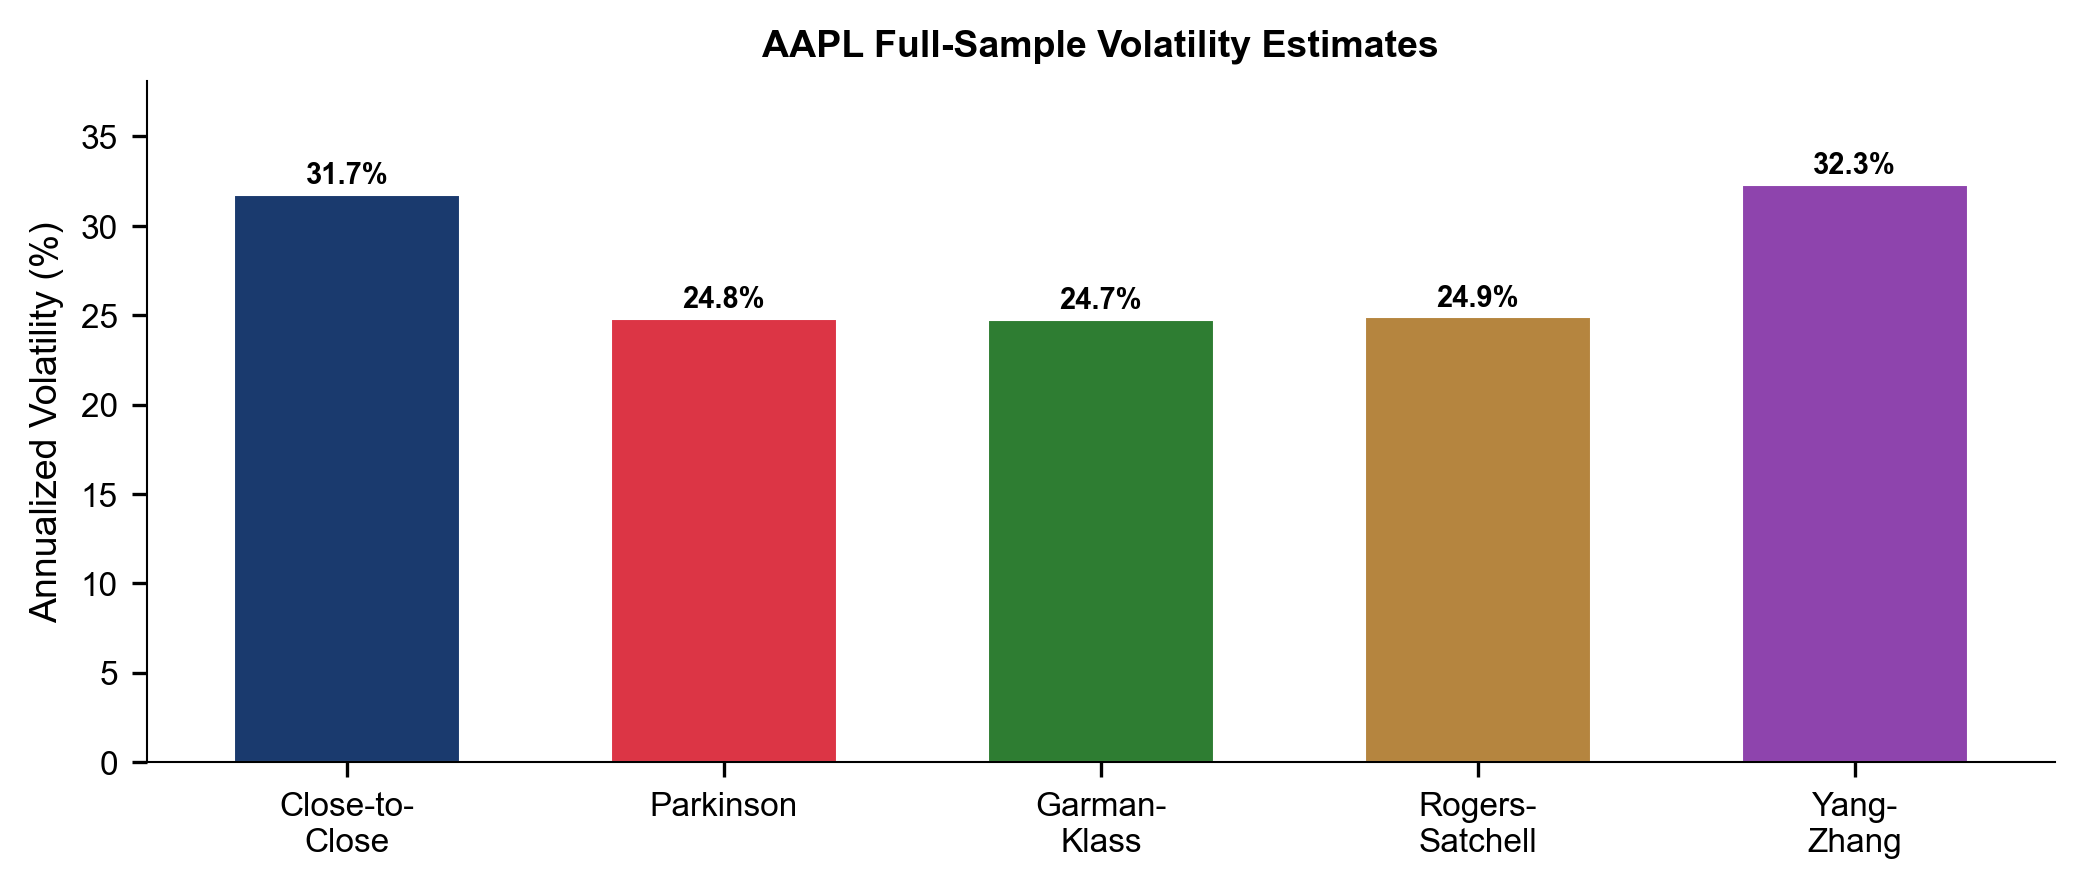
\includegraphics[width=\textwidth]{sfm_sem5_vol_barplot.png}
            {\tiny Comparație: estimatorii dau valori diferite pe aceleași date}
        \end{column}
    \end{columns}
    \quantlet{SFM\_ch1\_volatility\_estimators}{https://github.com/QuantLet/Stat_fin_markets/tree/master/Ch_01/SFM_ch1_volatility_estimators}
\end{cminipage}
\end{frame}

\begin{frame}[shrink=10]{Adevărat sau Fals? --- Întrebări (Partea II)}
\begin{cminipage}{0.95\textwidth}
    \begin{itemize}\setlength{\itemsep}{0pt}
        \item \textbf{Răspundeți cu Adevărat (A) sau Fals (F):}
    \end{itemize}
    \vspace{0.3cm}
    \begin{enumerate}\setlength{\itemsep}{0pt}
        \setcounter{enumi}{7}
        \item Indicatorul Sharpe este definit ca $SR = \bar{R} / \sigma$ (fără rata fără risc).
        \item Diversificarea reduce volatilitatea portofoliului doar dacă corelația este negativă.
        \item Volatilitatea portofoliului este medie ponderată a volatilităților individuale.
        \item Pe piețe 24/7 (crypto), Yang-Zhang converge la Rogers-Satchell.
        \item Un activ cu $SR = 2$ este considerat excelent.
        \item Autocorelația negativă a randamentelor face ca regula $\sqrt{T}$ să supraestimeze volatilitatea anuală.
        \item Portofoliul cu varianță minimă are întotdeauna cel mai mare Sharpe ratio.
    \end{enumerate}
\end{cminipage}
\end{frame}

\begin{frame}[shrink=10]{Adevărat sau Fals? --- Răspunsuri (Partea II)}
\begin{cminipage}{0.95\textwidth}
    \footnotesize
    \begin{enumerate}\setlength{\itemsep}{1pt}
        \setcounter{enumi}{7}
        \item \textcolor{Crimson}{\textbf{F}}: Formula corectă: $SR = (\bar{R} - R_f)/\sigma$; rata fără risc $R_f$ este esențială
        \item \textcolor{Crimson}{\textbf{F}}: Diversificarea funcționează pentru \textit{orice} $\rho < 1$; la $\rho = 0$, reducerea este $\sim 29\%$
        \item \textcolor{Crimson}{\textbf{F}}: $\sigma_p = \sqrt{\mathbf{w}^T \Sigma\, \mathbf{w}}$ include covarianțele; doar dacă $\rho = 1$ este medie ponderată
        \item \textcolor{Forest}{\textbf{A}}: Fără gap-uri: $O_t = C_{t-1}$ $\Rightarrow$ $\sigma_O^2 = 0$ $\Rightarrow$ $\sigma_{YZ}^2 \approx \sigma_{RS}^2$
        \item \textcolor{Forest}{\textbf{A}}: Scala interpretării: $< 0$ sub $R_f$; $0$--$0{,}5$ slab; $0{,}5$--$1$ acceptabil; $1$--$2$ bun; $> 2$ excelent
        \item \textcolor{Forest}{\textbf{A}}: Cu $\phi < 0$: factorul $(1+\phi)/(1-\phi) < 1$ $\Rightarrow$ regula $\sqrt{T}$ \textbf{supraestimează}
        \item \textcolor{Crimson}{\textbf{F}}: Portofoliul optim (Sharpe maxim) este pe frontiera eficientă, dar \textbf{nu} coincide cu cel de varianță minimă
    \end{enumerate}
\end{cminipage}
\end{frame}

%=============================================================================
% EXERCIȚII DE CALCUL
%=============================================================================
\section{Exerciții de Calcul}

\begin{frame}[shrink=20]{Exercițiul 1: Volatilitate Istorică}
    \begin{cminipage}{0.95\textwidth}
    \begin{block}{Enunț}
    \begin{center}
    {\small\renewcommand{\arraystretch}{1.3}
    \begin{tabular}{lcccccc}
    \toprule
    $t$ & 0 & 1 & 2 & 3 & 4 & 5 \\
    \midrule
    $P_t$ & 100 & 102 & 99 & 103 & 101 & 104 \\
    \bottomrule
    \end{tabular}}
    \end{center}
    Calculați randamentele logaritmice, volatilitatea istorică și anualizați-o.
    \end{block}
    \vspace{0.1cm}
    \begin{exampleblock}{Rezolvare}
    \begin{itemize}\setlength{\itemsep}{0pt}
        \item $r_1 = \ln(102/100) = 0{,}0198$, \; $r_2 = \ln(99/102) = -0{,}0299$, \; $r_3 = 0{,}0396$, \; $r_4 = -0{,}0196$, \; $r_5 = 0{,}0293$
        \item $\bar{r} = (0{,}0198 - 0{,}0299 + 0{,}0396 - 0{,}0196 + 0{,}0293)/5 = 0{,}00784$
        \item $\sigma = \sqrt{\frac{1}{4}\sum_{t=1}^{5}(r_t - \bar{r})^2} \approx 0{,}0290 = 2{,}90\%$
        \item $\sigma_{\text{anual}} = 2{,}90\% \times \sqrt{252} \approx \mathbf{46{,}0\%}$
    \end{itemize}
    \end{exampleblock}
    \begin{alertblock}{Interpretare economică}
    \begin{itemize}\setlength{\itemsep}{0pt}
        \item Volatilitatea anualizată de 46\% este \textbf{foarte mare} --- doar 5 observații produc un estimator instabil
        \item Comparați cu S\&P 500 ($\sigma \approx 16\%$): activul nostru ar fi de $\sim 3\times$ mai volatil
        \item Variance drag asociat: $\sigma^2/2 = 0{,}46^2/2 \approx 10{,}6\%$/an --- \textbf{distruge} randamentul
        \item \textbf{Concluzie practică}: cu 5 observații, estimatorul nu este fiabil; în practică se folosesc min.\ 30 zile
    \end{itemize}
    \end{alertblock}
    \end{cminipage}
\end{frame}

\begin{frame}[shrink=25]{Exercițiul 2: Estimatorul Parkinson}
    \begin{cminipage}{0.95\textwidth}
    \begin{block}{Enunț}
    \begin{center}
    {\small\renewcommand{\arraystretch}{1.3}
    \begin{tabular}{c c c}
    \toprule
    Ziua & $H_t$ & $L_t$ \\
    \midrule
    1 & 105 & 98 \\
    2 & 103 & 100 \\
    3 & 107 & 101 \\
    \bottomrule
    \end{tabular}}
    \end{center}
    Calculați estimatorul Parkinson al volatilității zilnice.
    \end{block}
    \vspace{0.1cm}
    \begin{exampleblock}{Rezolvare}
    \begin{itemize}\setlength{\itemsep}{0pt}
        \item $(\ln(H_1/L_1))^2 = (\ln(105/98))^2 = 0{,}0690^2 = 0{,}00476$
        \item $(\ln(H_2/L_2))^2 = (\ln(103/100))^2 = 0{,}0296^2 = 0{,}000877$
        \item $(\ln(H_3/L_3))^2 = (\ln(107/101))^2 = 0{,}0577^2 = 0{,}00333$
        \item $\sigma_P = \frac{1}{\sqrt{4\ln 2}}\sqrt{\frac{0{,}00476 + 0{,}000877 + 0{,}00333}{3}} = \frac{1}{1{,}665} \times 0{,}05467 \approx \mathbf{3{,}28\%}$ zilnic
    \end{itemize}
    \end{exampleblock}
    \begin{alertblock}{Interpretare}
    \begin{itemize}\setlength{\itemsep}{0pt}
        \item Anualizat: $3{,}28\% \times \sqrt{252} = 52{,}1\%$ --- asemănător cu acțiuni tech volatile sau crypto
        \item Parkinson surprinde mișcarea intra-zilnică ignorată de CC: ziua 1 are range $H/L = 7\%$!
        \item \textbf{Întrebare}: dacă prețul de închidere ar fi egal cu cel de deschidere în fiecare zi, CC ar da $\sigma = 0$, dar Parkinson $> 0$. De ce?
    \end{itemize}
    \end{alertblock}
    \end{cminipage}
\end{frame}

\begin{frame}[shrink=10]{Exercițiul 3: Scalarea Volatilității}
    \begin{cminipage}{0.95\textwidth}
    \begin{block}{Enunț: O acțiune are volatilitate zilnică de $1{,}5\%$. Scalați.}
    \end{block}
    \vspace{0.1cm}
    \begin{columns}[T]
    \begin{column}{0.48\textwidth}
    \begin{exampleblock}{Rezolvare}
    \begin{itemize}\setlength{\itemsep}{0pt}
        \item $\sigma_{\text{săpt}} = 1{,}5\% \times \sqrt{5} = \mathbf{3{,}35\%}$
        \item $\sigma_{\text{lunar}} = 1{,}5\% \times \sqrt{22} = \mathbf{7{,}04\%}$
        \item $\sigma_{\text{anual}} = 1{,}5\% \times \sqrt{252} = \mathbf{23{,}81\%}$
    \end{itemize}
    \end{exampleblock}
    \end{column}
    \begin{column}{0.50\textwidth}
    \begin{center}
    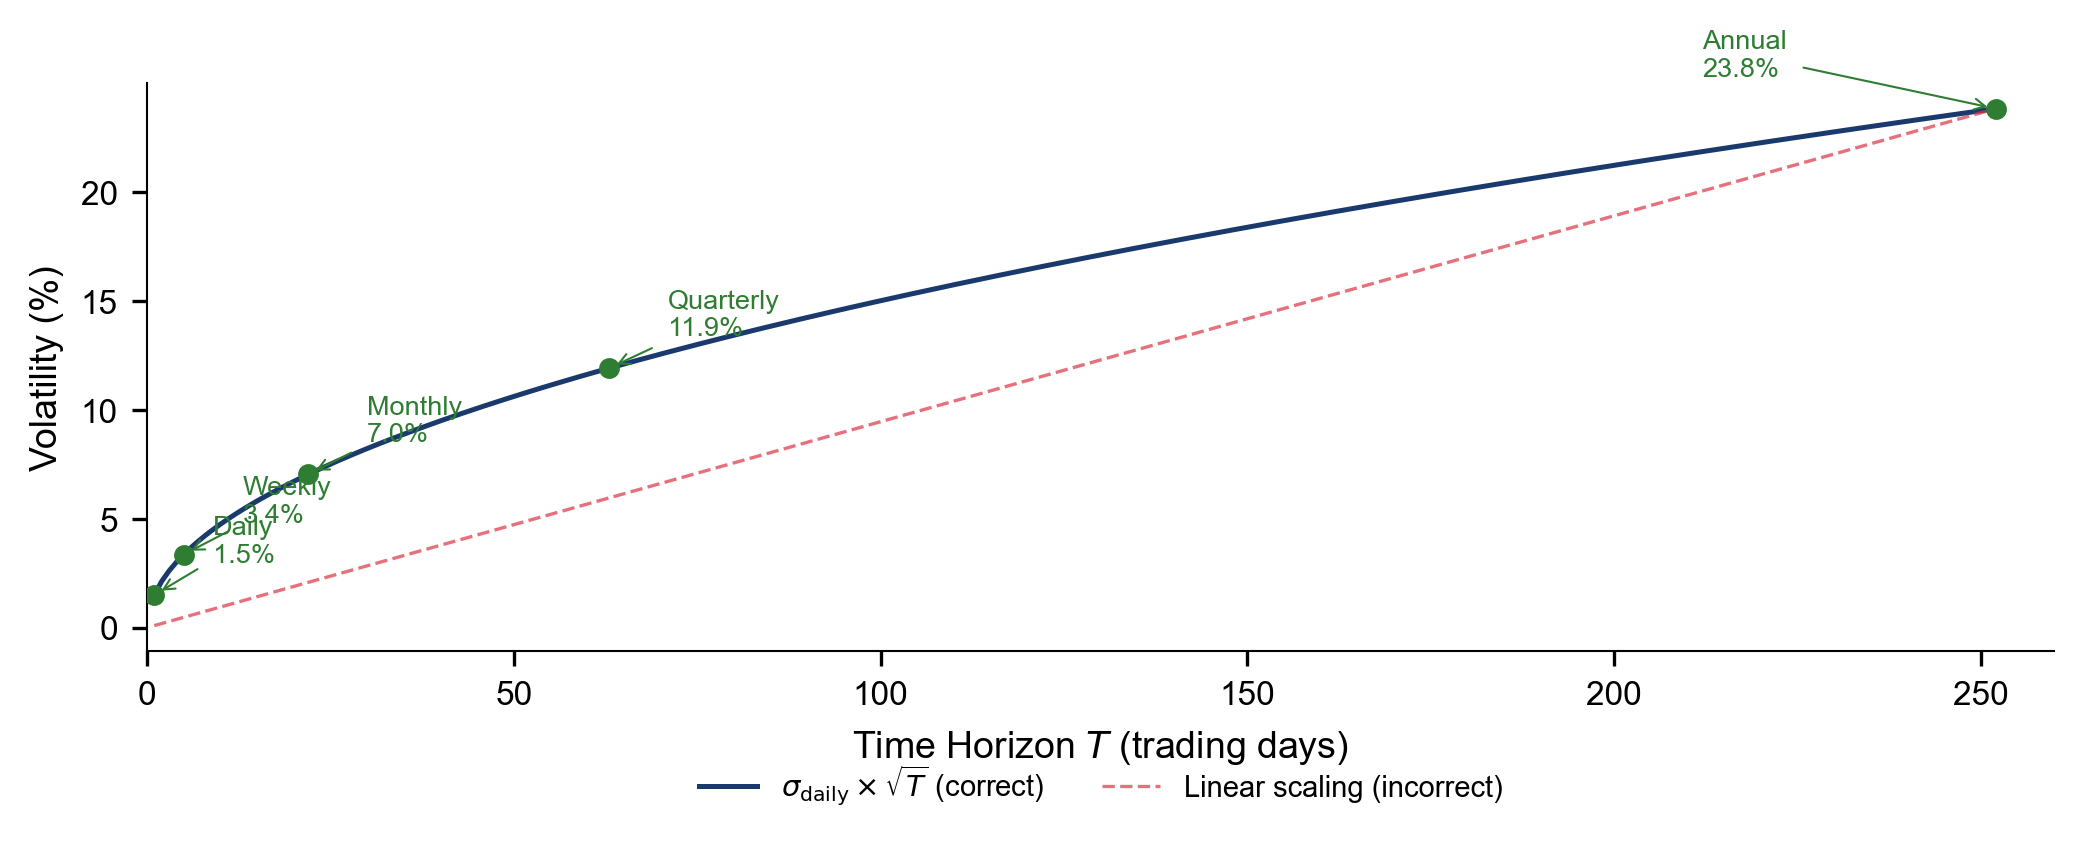
\includegraphics[width=\linewidth]{sfm_sem5_sqrt_time.png}
    \end{center}
    \end{column}
    \end{columns}
    \vspace{0.1cm}
    \begin{alertblock}{Interpretare economică și comparație}
    \begin{itemize}\setlength{\itemsep}{0pt}
        \item Volatilitatea crește \textbf{subliniar} cu timpul ($\sqrt{T}$), varianța crește \textbf{liniar} ($T$)
        \item $\sigma_{\text{anual}} = 23{,}81\%$: apropiat de S\&P 500 ($\sim$16\%) --- activ moderat volatil
        \item Variance drag: $0{,}2381^2/2 = 2{,}83\%$/an --- pentru un fond cu $\mu = 8\%$, creșterea reală $\approx 5{,}2\%$
        \item \textbf{Comparați}: BTC ($\sigma \approx 70\%$) $\Rightarrow$ drag $= 24{,}5\%$ --- volatilitatea mare e costisitoare!
    \end{itemize}
    \end{alertblock}
    \quantlet{SFM\_ch1\_volatility\_estimators}{https://github.com/QuantLet/Stat_fin_markets/tree/master/Ch_01/SFM_ch1_volatility_estimators}
    \end{cminipage}
\end{frame}

\begin{frame}[shrink=10]{Exercițiul 4: Garman-Klass}
    \begin{cminipage}{0.95\textwidth}
    \begin{block}{Enunț: $O = 100$, $H = 105$, $L = 97$, $C = 103$. Calculați $\sigma_{GK}$.}
    \end{block}
    \vspace{0.1cm}
    \begin{exampleblock}{Rezolvare}
    \begin{itemize}\setlength{\itemsep}{0pt}
        \item $\ln(H/L) = \ln(105/97) = 0{,}0792$, \quad $(\ln(H/L))^2 = 0{,}006273$
        \item $\ln(C/O) = \ln(103/100) = 0{,}0296$, \quad $(\ln(C/O))^2 = 0{,}000877$
        \item $\sigma_{GK}^2 = 0{,}5 \times 0{,}006273 - (2\ln 2 - 1) \times 0{,}000877$
        \item $2\ln 2 - 1 = 0{,}3863$
        \item $\sigma_{GK}^2 = 0{,}003137 - 0{,}000339 = 0{,}002798$
        \item $\sigma_{GK} = \sqrt{0{,}002798} \approx \mathbf{5{,}29\%}$ (volatilitate zilnică)
    \end{itemize}
    \end{exampleblock}
    \end{cminipage}
\end{frame}

\begin{frame}[shrink=10]{Exercițiul 5: Rogers-Satchell}
    \begin{cminipage}{0.95\textwidth}
    \begin{block}{Enunț: Aceleași date OHLC: $O = 100$, $H = 105$, $L = 97$, $C = 103$. Calculați $\sigma_{RS}$.}
    \end{block}
    \vspace{0.1cm}
    \begin{exampleblock}{Rezolvare}
    \begin{itemize}\setlength{\itemsep}{0pt}
        \item $u = \ln(H/O) = \ln(105/100) = 0{,}04879$
        \item $d = \ln(L/O) = \ln(97/100) = -0{,}03046$
        \item $c = \ln(C/O) = \ln(103/100) = 0{,}02956$
        \item $\sigma_{RS}^2 = u(u - c) + d(d - c)$
        \item $= 0{,}04879 \times 0{,}01923 + (-0{,}03046) \times (-0{,}06002) = 0{,}000938 + 0{,}001828 = 0{,}002766$
        \item $\sigma_{RS} = \sqrt{0{,}002766} \approx \mathbf{5{,}26\%}$
    \end{itemize}
    \end{exampleblock}
    \begin{alertblock}{Comparație GK vs RS}
    \begin{itemize}\setlength{\itemsep}{0pt}
        \item GK = 5,29\% vs RS = 5,26\% --- valori apropiate pe aceste date
        \item Diferența crește când drift-ul este semnificativ (RS este robust la drift)
    \end{itemize}
    \end{alertblock}
    \end{cminipage}
\end{frame}

\begin{frame}[shrink=20]{Exercițiul 6: Comparație pe fereastră de 3 zile}
    \begin{cminipage}{0.95\textwidth}
    \begin{block}{Enunț}
    \begin{center}
    {\small\renewcommand{\arraystretch}{1.3}
    \begin{tabular}{c c c c c}
    \toprule
    Ziua & $O_t$ & $H_t$ & $L_t$ & $C_t$ \\
    \midrule
    1 & 100 & 104 & 98 & 102 \\
    2 & 102 & 106 & 100 & 101 \\
    3 & 101 & 105 & 99 & 104 \\
    \bottomrule
    \end{tabular}}
    \end{center}
    Calculați volatilitatea close-to-close și Parkinson.
    \end{block}
    \vspace{0.1cm}
    \begin{columns}[T]
    \begin{column}{0.48\textwidth}
    \begin{exampleblock}{Close-to-Close}
    \begin{itemize}\setlength{\itemsep}{0pt}
        \item $r_1 = \ln(102/100) = 0{,}0198$
        \item $r_2 = \ln(101/102) = -0{,}0099$
        \item $r_3 = \ln(104/101) = 0{,}0293$
        \item $\bar{r} = 0{,}01307$, \; $\sigma \approx \mathbf{2{,}01\%}$
    \end{itemize}
    \end{exampleblock}
    \end{column}
    \begin{column}{0.48\textwidth}
    \begin{exampleblock}{Parkinson}
    \begin{itemize}\setlength{\itemsep}{0pt}
        \item $(\ln(104/98))^2 = 0{,}00354$
        \item $(\ln(106/100))^2 = 0{,}00340$
        \item $(\ln(105/99))^2 = 0{,}00351$
        \item $\sigma_P \approx \mathbf{2{,}18\%}$
    \end{itemize}
    \end{exampleblock}
    \end{column}
    \end{columns}
    \vspace{0.1cm}
    \begin{alertblock}{Concluzie}
    \begin{itemize}\setlength{\itemsep}{0pt}
        \item Parkinson estimează volatilitate \textbf{mai mare} deoarece surprinde mișcările \textbf{intra-zilnice}
    \end{itemize}
    \end{alertblock}
    \end{cminipage}
\end{frame}

\begin{frame}[shrink=10]{Exercițiul 7: De unde vine constanta $\frac{1}{\sqrt{4\ln 2}}$?}
    \begin{cminipage}{0.95\textwidth}
    \begin{block}{Enunț}
    \begin{itemize}\setlength{\itemsep}{0pt}
        \item Parkinson (1980) presupune că log-prețul urmează un random walk: $\ln P_t = \ln P_{t-1} + \sigma\,\varepsilon_t$, $\varepsilon_t \sim \mathcal{N}(0,1)$.
        \item Sub acest model, se poate demonstra că $\E\!\left[\left(\ln\frac{H}{L}\right)^{\!2}\right] = 4\ln 2 \cdot \sigma^2$.
        \item Verificați numeric această relație prin simulare Monte Carlo (exercițiu Python).
    \end{itemize}
    \end{block}
    \vspace{0.1cm}
    \begin{exampleblock}{Explicație intuitivă}
    \begin{itemize}\setlength{\itemsep}{0pt}
        \item Intervalul $\ln(H/L)$ captează \textbf{toată variația} intra-zilnică, nu doar punctele de la Open/Close
        \item Valoarea așteptată a pătratului intervalului este proporțională cu $\sigma^2$, cu factorul $4\ln 2 \approx 2{,}773$
        \item Inversând: $\hat{\sigma}^2 = \frac{1}{4\ln 2}\left(\ln\frac{H}{L}\right)^{\!2}$ --- estimator nedeplasat
        \item Folosește \textbf{mai multă informație} decât close-to-close $\Rightarrow$ de $\sim$5$\times$ mai eficient
        \item \textbf{Limitare}: presupune tranzacționare continuă (fără gap-uri, fără salturi de preț)
    \end{itemize}
    \end{exampleblock}
    \end{cminipage}
\end{frame}

\begin{frame}[shrink=10]{Exercițiul 8: Autocorelație și regula $\sqrt{T}$}
    \begin{cminipage}{0.95\textwidth}
    \begin{block}{Enunț}
    \begin{itemize}\setlength{\itemsep}{0pt}
        \item Fie $r_t$ un proces AR(1): $r_t = \phi\, r_{t-1} + \varepsilon_t$, $\varepsilon_t \sim (0, \sigma_\varepsilon^2)$, $|\phi| < 1$.
        \item Derivați $\Var(R_n)$ unde $R_n = \sum_{t=1}^n r_t$ și arătați că diferă de $n\sigma^2$.
    \end{itemize}
    \end{block}
    \vspace{0.1cm}
    \begin{exampleblock}{Rezolvare}
    \begin{itemize}\setlength{\itemsep}{0pt}
        \item $\sigma^2 = \Var(r_t) = \sigma_\varepsilon^2 / (1 - \phi^2)$, \quad $\gamma_k = \Cov(r_t, r_{t+k}) = \sigma^2 \phi^k$
        \item $\Var(R_n) = n\sigma^2 + 2\sum_{k=1}^{n-1}(n-k)\sigma^2\phi^k = n\sigma^2\!\left[1 + \frac{2\phi}{1-\phi}\!\left(1 - \frac{1-\phi^n}{n(1-\phi)}\right)\right]$
        \item Pentru $n$ mare: $\Var(R_n) \approx n\sigma^2 \cdot \frac{1+\phi}{1-\phi}$
        \item \textbf{Exemplu numeric:} $\phi = 0{,}3$, $\sigma = 1\%$:
        \begin{itemize}\setlength{\itemsep}{0pt}
            \item Regula $\sqrt{T}$: $\sigma_{252} = 1\% \times \sqrt{252} = 15{,}87\%$
            \item Corect: $\sigma_{252} \approx 15{,}87\% \times \sqrt{1{,}3/0{,}7} = 15{,}87\% \times 1{,}363 = \mathbf{21{,}63\%}$
            \item Subestimarea: $\approx 36\%$ --- semnificativă!
        \end{itemize}
    \end{itemize}
    \end{exampleblock}
    \end{cminipage}
\end{frame}

\begin{frame}[shrink=15]{Indicatorul Sharpe}
    \begin{cminipage}{0.95\textwidth}
    \begin{columns}[T]
    \begin{column}{0.48\textwidth}
    \begin{block}{Definiție}
    \begin{itemize}\setlength{\itemsep}{0pt}
        \item Măsoară \textbf{randamentul excesiv} față de rata fără risc, ajustat pentru volatilitate:
        \[
        SR = \frac{\bar{R} - R_f}{\sigma}
        \]
        \item $\bar{R}$: randamentul mediu al activului
        \item $R_f$: rata fără risc (obligațiuni de stat)
        \item $\sigma$: volatilitatea randamentelor
    \end{itemize}
    \end{block}
    \end{column}
    \begin{column}{0.48\textwidth}
    \begin{center}
    {\small\renewcommand{\arraystretch}{1.2}
    \begin{tabular}{>{\centering\arraybackslash}p{1.5cm} >{\centering\arraybackslash}p{2cm}}
    \toprule
    \textbf{Sharpe} & \textbf{Interpretare} \\
    \midrule
    \rowcolor{Crimson!30} $SR < 0$ & Sub rata fără risc \\
    \rowcolor{Orange!30} $0 - 0{,}5$ & Slab \\
    \rowcolor{Amber!30} $0{,}5 - 1$ & Acceptabil \\
    \rowcolor{Forest!20} $1 - 2$ & Bun \\
    \rowcolor{Forest!40} $> 2$ & Excelent \\
    \bottomrule
    \end{tabular}}
    \end{center}
    \end{column}
    \end{columns}
    \end{cminipage}
\end{frame}

\begin{frame}[shrink=10]{Volatilitatea portofoliului și frontiera eficientă}
    \begin{cminipage}{0.95\textwidth}
    \begin{columns}[T]
    \begin{column}{0.48\textwidth}
    \begin{block}{Volatilitatea portofoliului}
    \begin{itemize}\setlength{\itemsep}{0pt}
        \item Ține cont de \textbf{corelațiile dintre active}:
        \[
        \sigma_p = \sqrt{\mathbf{w}^T \Sigma\, \mathbf{w}}
        \]
        \item $\mathbf{w}$: vectorul ponderilor
        \item $\Sigma$: matricea de covarianță
        \item Anualizat: $\sigma_{\text{anual}} = \sigma_{\text{zilnic}} \times \sqrt{252}$
    \end{itemize}
    \end{block}
    \end{column}
    \begin{column}{0.48\textwidth}
    \begin{exampleblock}{Frontiera eficientă}
    \begin{itemize}\setlength{\itemsep}{0pt}
        \item Portofolii care \textbf{maximizează} randamentul pentru un nivel dat de risc
        \item Sau \textbf{minimizează} riscul pentru un randament dat
        \item Portofoliul \textbf{optim}: maximizează Sharpe
        \item Sub frontieră = suboptimal
    \end{itemize}
    \end{exampleblock}
    \end{column}
    \end{columns}
    \vspace{0.2cm}
    \begin{alertblock}{Randamentul așteptat al portofoliului}
    \begin{itemize}\setlength{\itemsep}{0pt}
        \item $\E[R_p] = \sum_{i=1}^n w_i \cdot \E[R_i]$ --- media ponderată a randamentelor individuale
        \item Diversificarea reduce $\sigma_p$ (dacă $\rho < 1$) dar \textbf{nu} reduce $\E[R_p]$
    \end{itemize}
    \end{alertblock}
    \end{cminipage}
\end{frame}

\begin{frame}[shrink=15]{Exercițiul 9: Sharpe și portofoliu}
    \begin{cminipage}{0.95\textwidth}
    \begin{block}{Enunț}
    \begin{center}
    {\small\renewcommand{\arraystretch}{1.2}
    \begin{tabular}{lcccc}
    \toprule
    \textbf{Activ} & $\E[R]$ (\%) & $\sigma$ (\%) & \textbf{Sharpe} ($R_f = 2\%$) \\
    \midrule
    SPY & 14{,}33 & 19{,}35 & ? \\
    QQQ & 19{,}57 & 24{,}04 & ? \\
    GLD & 11{,}62 & 14{,}31 & ? \\
    \bottomrule
    \end{tabular}}
    \end{center}
    Calculați Sharpe pentru fiecare. Apoi: un portofoliu 50\% SPY + 50\% GLD cu $\rho = 0{,}15$. Calculați $\sigma_p$ și $SR_p$.
    \end{block}
    \vspace{0.1cm}
    \begin{exampleblock}{Rezolvare}
    \begin{itemize}\setlength{\itemsep}{0pt}
        \item $SR_{\text{SPY}} = (14{,}33 - 2)/19{,}35 = \mathbf{0{,}637}$; \; $SR_{\text{QQQ}} = (19{,}57 - 2)/24{,}04 = \mathbf{0{,}731}$; \; $SR_{\text{GLD}} = (11{,}62 - 2)/14{,}31 = \mathbf{0{,}672}$
        \item Portofoliu: $\E[R_p] = 0{,}5 \times 14{,}33 + 0{,}5 \times 11{,}62 = 12{,}98\%$
        \item $\sigma_p = \sqrt{0{,}5^2 \times 19{,}35^2 + 0{,}5^2 \times 14{,}31^2 + 2 \times 0{,}5 \times 0{,}5 \times 19{,}35 \times 14{,}31 \times 0{,}15} = \mathbf{13{,}17\%}$
        \item $SR_p = (12{,}98 - 2)/13{,}17 = \mathbf{0{,}833}$ --- mai bun decât oricare activ individual!
    \end{itemize}
    \end{exampleblock}
    \begin{alertblock}{Concluzie}
    \begin{itemize}\setlength{\itemsep}{0pt}
        \item Diversificarea a redus $\sigma$ de la $\sim$17\% (medie) la 13{,}17\% și a crescut Sharpe cu $\sim$20\%
    \end{itemize}
    \end{alertblock}
    \end{cminipage}
\end{frame}

\begin{frame}[shrink=15]{Exercițiul 10: Derivarea volatilității portofoliului (2 active)}
    \begin{cminipage}{0.95\textwidth}
    \begin{block}{Enunț}
    \begin{itemize}\setlength{\itemsep}{0pt}
        \item Un portofoliu din activele X și Y cu ponderi $w_X$ și $w_Y = 1 - w_X$.
        \item Volatilități: $\sigma_X = 25\%$, $\sigma_Y = 15\%$, corelație $\rho_{XY} = -0{,}3$.
        \item Derivați formula $\sigma_p$ și calculați pentru $w_X = 0{,}6$.
    \end{itemize}
    \end{block}
    \vspace{0.1cm}
    \begin{exampleblock}{Rezolvare}
    \begin{itemize}\setlength{\itemsep}{0pt}
        \item $\sigma_p^2 = w_X^2\sigma_X^2 + w_Y^2\sigma_Y^2 + 2\,w_X\,w_Y\,\sigma_X\,\sigma_Y\,\rho_{XY}$
        \item $= 0{,}6^2 \times 0{,}25^2 + 0{,}4^2 \times 0{,}15^2 + 2 \times 0{,}6 \times 0{,}4 \times 0{,}25 \times 0{,}15 \times (-0{,}3)$
        \item $= 0{,}0225 + 0{,}0036 - 0{,}0054 = 0{,}0207$
        \item $\sigma_p = \sqrt{0{,}0207} = \mathbf{14{,}39\%}$
    \end{itemize}
    \end{exampleblock}
    \begin{alertblock}{Interpretare}
    \begin{itemize}\setlength{\itemsep}{0pt}
        \item Media ponderată ar fi $0{,}6 \times 25 + 0{,}4 \times 15 = 21\%$, dar $\sigma_p = 14{,}39\%$ --- reducere de \textbf{31\%}!
        \item Corelația negativă ($\rho = -0{,}3$) amplifică efectul diversificării
        \item \textbf{Exercițiu}: ce se întâmplă dacă $\rho = +0{,}9$? Dar dacă $\rho = -1$?
    \end{itemize}
    \end{alertblock}
    \end{cminipage}
\end{frame}

\begin{frame}[shrink=10]{Exercițiul 11: Efectul corelației asupra diversificării}
    \begin{cminipage}{0.95\textwidth}
    \begin{block}{Enunț}
    \begin{itemize}\setlength{\itemsep}{0pt}
        \item Două active cu $\sigma_A = \sigma_B = 20\%$, portofoliu echilibrat $w_A = w_B = 0{,}5$.
        \item Calculați $\sigma_p$ pentru $\rho \in \{-1,\; -0{,}5,\; 0,\; 0{,}5,\; 1\}$.
    \end{itemize}
    \end{block}
    \vspace{0.1cm}
    \begin{exampleblock}{Rezolvare}
    \begin{center}
    {\small\renewcommand{\arraystretch}{1.2}
    \begin{tabular}{cccccc}
    \toprule
    $\rho$ & $-1$ & $-0{,}5$ & $0$ & $0{,}5$ & $1$ \\
    \midrule
    $\sigma_p$ & $0\%$ & $10{,}0\%$ & $14{,}14\%$ & $17{,}32\%$ & $20{,}0\%$ \\
    \textbf{Reducere} & $-100\%$ & $-50\%$ & $-29\%$ & $-13\%$ & $0\%$ \\
    \bottomrule
    \end{tabular}}
    \end{center}
    \end{exampleblock}
    \begin{alertblock}{Concluzie}
    \begin{itemize}\setlength{\itemsep}{0pt}
        \item La $\rho = -1$: risc \textbf{zero} (hedging perfect) --- în practică nu există
        \item La $\rho = 0$: reducere de 29\% --- diversificarea funcționează chiar fără corelație negativă
        \item La $\rho = 1$: \textbf{niciun beneficiu} --- activele se mișcă identic
        \item \textbf{Lecție}: căutăm active cu corelație \textbf{scăzută}, nu neapărat negativă
    \end{itemize}
    \end{alertblock}
    \end{cminipage}
\end{frame}

\begin{frame}[shrink=10]{Exercițiul 12: Sharpe și portofoliu cu 3 active (I)}
    \begin{cminipage}{0.95\textwidth}
    \begin{block}{Enunț}
    \begin{itemize}\setlength{\itemsep}{0pt}
        \item Trei active cu următoarele caracteristici ($R_f = 2\%$):
    \end{itemize}
    \begin{center}
    {\small\renewcommand{\arraystretch}{1.2}
    \begin{tabular}{lccc}
    \toprule
    \textbf{Activ} & $\E[R]$ (\%) & $\sigma$ (\%) & $SR$ \\
    \midrule
    Acțiuni (A) & 12 & 22 & ? \\
    Obligațiuni (B) & 5 & 8 & ? \\
    Mărfuri (C) & 9 & 18 & ? \\
    \bottomrule
    \end{tabular}}
    \end{center}
    \begin{itemize}\setlength{\itemsep}{0pt}
        \item Matricea de corelație:
    \end{itemize}
    \begin{center}
    {\small
    $\rho = \begin{pmatrix} 1 & -0{,}2 & 0{,}4 \\ -0{,}2 & 1 & 0{,}1 \\ 0{,}4 & 0{,}1 & 1 \end{pmatrix}$}
    \end{center}
    \begin{itemize}\setlength{\itemsep}{0pt}
        \item \textbf{(a)} Calculați Sharpe ratio pentru fiecare activ
        \item \textbf{(b)} Un portofoliu cu ponderi $w_A = 0{,}5$, $w_B = 0{,}3$, $w_C = 0{,}2$ --- calculați $\E[R_p]$, $\sigma_p$ și $SR_p$
    \end{itemize}
    \end{block}
    \end{cminipage}
\end{frame}

\begin{frame}[shrink=10]{Exercițiul 12: Sharpe și portofoliu cu 3 active (II)}
    \begin{cminipage}{0.95\textwidth}
    \begin{exampleblock}{Rezolvare (a): Sharpe ratio individual}
    \begin{itemize}\setlength{\itemsep}{0pt}
        \item $SR_A = \frac{12 - 2}{22} = \frac{10}{22} = \mathbf{0{,}455}$
        \item $SR_B = \frac{5 - 2}{8} = \frac{3}{8} = \mathbf{0{,}375}$
        \item $SR_C = \frac{9 - 2}{18} = \frac{7}{18} = \mathbf{0{,}389}$
        \item Acțiunile au cel mai mare Sharpe, urmate de mărfuri, apoi obligațiuni
    \end{itemize}
    \end{exampleblock}
    \vspace{0.1cm}
    \begin{exampleblock}{Rezolvare (b): Randamentul și volatilitatea portofoliului}
    \begin{itemize}\setlength{\itemsep}{0pt}
        \item $\E[R_p] = 0{,}5 \times 12 + 0{,}3 \times 5 + 0{,}2 \times 9 = 6 + 1{,}5 + 1{,}8 = \mathbf{9{,}3\%}$
        \item $\sigma_p^2 = 121{,}00 + 5{,}76 + 12{,}96 - 10{,}56 + 31{,}68 + 1{,}73 = 162{,}57$
        \item $\sigma_p = \sqrt{162{,}57} = \mathbf{12{,}75\%}$
    \end{itemize}
    \end{exampleblock}
    \begin{alertblock}{Sharpe ratio al portofoliului}
    \begin{itemize}\setlength{\itemsep}{0pt}
        \item $SR_p = \frac{9{,}3 - 2}{12{,}75} = \mathbf{0{,}573}$ --- mai bun decât oricare activ individual!
        \item Media ponderată a volatilităților: $0{,}5 \times 22 + 0{,}3 \times 8 + 0{,}2 \times 18 = 17\%$, dar $\sigma_p = 12{,}75\%$ --- reducere de \textbf{25\%}
    \end{itemize}
    \end{alertblock}
    \end{cminipage}
\end{frame}

\begin{frame}[shrink=10]{Exercițiul 13: Portofoliul cu varianță minimă}
    \begin{cminipage}{0.95\textwidth}
    \begin{block}{Enunț}
    \begin{itemize}\setlength{\itemsep}{0pt}
        \item Două active A și B cu volatilitățile $\sigma_A = 30\%$, $\sigma_B = 20\%$, corelația $\rho = 0{,}2$.
        \item Derivați ponderea $w_A^*$ care minimizează $\sigma_p$ și calculați $\sigma_p^{\min}$.
    \end{itemize}
    \end{block}
    \vspace{0.1cm}
    \begin{exampleblock}{Rezolvare}
    \begin{itemize}\setlength{\itemsep}{0pt}
        \item $w^* = \frac{\sigma_B^2 - \rho\,\sigma_A\,\sigma_B}{\sigma_A^2 + \sigma_B^2 - 2\,\rho\,\sigma_A\,\sigma_B} = \frac{0{,}04 - 0{,}012}{0{,}09 + 0{,}04 - 0{,}024} = \frac{0{,}028}{0{,}106} = \mathbf{0{,}264}$
        \item $w_B^* = 1 - 0{,}264 = \mathbf{0{,}736}$
        \item $\sigma_p^2 = 0{,}264^2 \times 0{,}09 + 0{,}736^2 \times 0{,}04 + 2 \times 0{,}264 \times 0{,}736 \times 0{,}06 \times 0{,}2 = 0{,}03261$
        \item $\sigma_p^{\min} = \sqrt{0{,}03261} = \mathbf{18{,}06\%}$
    \end{itemize}
    \end{exampleblock}
    \begin{alertblock}{Interpretare}
    \begin{itemize}\setlength{\itemsep}{0pt}
        \item Activul mai puțin volatil (B) primește o pondere mai mare (73{,}6\%)
        \item $\sigma_p^{\min} = 18{,}06\% < \sigma_B = 20\%$ --- chiar sub volatilitatea celui mai stabil activ!
        \item Diversificarea este „gratis": reduce riscul fără a necesita predicții de randament
    \end{itemize}
    \end{alertblock}
    \end{cminipage}
\end{frame}

%=============================================================================
% EXERCIȚII PYTHON
%=============================================================================
\section{Exerciții Python}

\begin{frame}[shrink=10]{Exercițiu Python 1: Volatilitate istorică mobilă}
\begin{cminipage}{0.95\textwidth}
    \begin{block}{Sarcină}
    \begin{enumerate}\setlength{\itemsep}{0pt}
        \item Descărcați datele OHLC ale AAPL pe 2020--2025 cu \texttt{yfinance}
        \item Calculați log-randamentele și volatilitatea close-to-close mobilă pe 30 de zile
        \item Anualizați volatilitatea ($\times \sqrt{252}$)
        \item Vizualizați: prețul și volatilitatea pe 2 subgrafice
    \end{enumerate}
    \end{block}

    \vspace{0.2cm}
    \begin{alertblock}{Funcții cheie}
    \begin{itemize}\setlength{\itemsep}{0pt}
        \item \texttt{yf.download(ticker, start, end)} --- descărcare date
        \item \texttt{np.log(data['Close'] / data['Close'].shift(1))} --- log-randamente
        \item \texttt{.rolling(30).std() * np.sqrt(252)} --- volatilitate mobilă anualizată
    \end{itemize}
    \end{alertblock}

    \quantlet{SFM\_ch1\_volatility\_estimators}{https://github.com/QuantLet/Stat_fin_markets/tree/master/Ch_01/SFM_ch1_volatility_estimators}
\end{cminipage}
\end{frame}

\begin{frame}[shrink=10]{Exercițiu Python 2: Estimatori bazați pe intervale}
\begin{cminipage}{0.95\textwidth}
    \begin{block}{Sarcină}
    \begin{enumerate}\setlength{\itemsep}{0pt}
        \item Implementați funcții pentru estimatorii Parkinson, Garman-Klass, Rogers-Satchell și Yang-Zhang
        \item Aplicați pe datele AAPL cu fereastră mobilă de 30 de zile
        \item Vizualizați comparativ toți estimatorii pe același grafic
    \end{enumerate}
    \end{block}

    \vspace{0.2cm}
    \begin{alertblock}{Constante cheie de verificat}
    \begin{itemize}\setlength{\itemsep}{0pt}
        \item Parkinson: factorul $\frac{1}{4\ln 2}$ provine din $\E[(\ln H/L)^2]$ sub random walk
        \item GK: coeficientul $(2\ln 2 - 1) \approx 0{,}386$ ponderează componenta close-open
        \item YZ: $k = \frac{0{,}34}{1{,}34 + (n+1)/(n-1)}$ --- pondere optimală
        \item \textbf{Atenție}: \texttt{.clip(lower=0)} necesar înainte de $\sqrt{\cdot}$ (valori negative posibile numeric)
    \end{itemize}
    \end{alertblock}

    \quantlet{SFM\_ch1\_volatility\_estimators}{https://github.com/QuantLet/Stat_fin_markets/tree/master/Ch_01/SFM_ch1_volatility_estimators}
\end{cminipage}
\end{frame}

\begin{frame}[shrink=10]{Exercițiu Python 3: Comparație multi-active}
\begin{cminipage}{0.95\textwidth}
    \begin{block}{Sarcină}
    \begin{enumerate}\setlength{\itemsep}{0pt}
        \item Descărcați date pentru AAPL, SPY și BTC-USD
        \item Calculați volatilitatea CC și YZ pe 30 de zile pentru fiecare activ
        \item Comparați: unde diferă cel mai mult CC și YZ? De ce?
        \item Testați fereastra de estimare: 10, 30, 60 de zile --- care este trade-off-ul?
    \end{enumerate}
    \end{block}

    \vspace{0.2cm}
    \begin{exampleblock}{Rezultate așteptate}
    \begin{itemize}\setlength{\itemsep}{0pt}
        \item \textbf{BTC}: $\sim$60--80\% anualizat; CC $\approx$ YZ (piață 24/7, fără gap-uri)
        \item \textbf{AAPL}: $\sim$25--35\%; YZ $>$ CC (gap-uri overnight din rapoartele trimestriale)
        \item \textbf{SPY}: $\sim$15--20\%; diferență moderată CC vs YZ
        \item Fereastră mică $\Rightarrow$ reactiv, dar zgomot mare; fereastră mare $\Rightarrow$ neted, dar întârziat
    \end{itemize}
    \end{exampleblock}

    \quantlet{SFM\_ch1\_volatility\_estimators}{https://github.com/QuantLet/Stat_fin_markets/tree/master/Ch_01/SFM_ch1_volatility_estimators}
\end{cminipage}
\end{frame}

\begin{frame}[shrink=10]{Exercițiu Python 4: Frontiera eficientă cu Monte Carlo}
\begin{cminipage}{0.95\textwidth}
    \begin{block}{Sarcină}
    \begin{enumerate}\setlength{\itemsep}{0pt}
        \item Descărcați date pentru 5 active: SPY, QQQ, GLD, TLT, VNQ (2018--2025)
        \item Generați 10\,000 portofolii aleatorii (\texttt{np.random.dirichlet})
        \item Calculați randamentul, volatilitatea și Sharpe ratio pentru fiecare
        \item Vizualizați frontiera eficientă (scatter plot colorat după Sharpe)
        \item Identificați portofoliul optim (Sharpe maxim)
    \end{enumerate}
    \end{block}

    \vspace{0.2cm}
    \begin{alertblock}{Rezultate așteptate}
    \begin{itemize}\setlength{\itemsep}{0pt}
        \item Portofoliul optim: SPY $\approx 48\%$, QQQ $\approx 33\%$, GLD $\approx 17\%$
        \item $SR_{\text{optim}} \approx 0{,}91$ --- mai bun decât orice activ individual
        \item GLD intră 17\% deși are cel mai mic randament --- \textbf{corelație scăzută}!
        \item TLT ($SR < 0$) intră minimal --- diversificare marginală
    \end{itemize}
    \end{alertblock}

    \quantlet{SFM\_ch1\_volatility\_estimators}{https://github.com/QuantLet/Stat_fin_markets/tree/master/Ch_01/SFM_ch1_volatility_estimators}
\end{cminipage}
\end{frame}

%=============================================================================
% ÎNTREBĂRI DE DISCUȚIE
%=============================================================================
\section{Întrebări de Discuție}

\begin{frame}[shrink=10]{Discuție 1: Alegerea estimatorului în practică}
\begin{cminipage}{0.95\textwidth}
    \begin{itemize}\setlength{\itemsep}{0pt}
        \item \textbf{Scenariu:} Sunteți analist de risc într-un fond de investiții. Managerul vă cere estimarea volatilității pentru: acțiuni (NYSE), FX (EUR/USD, 24/5) și crypto (BTC, 24/7).
        \item \textbf{Întrebări:}
    \end{itemize}
    \begin{enumerate}\setlength{\itemsep}{0pt}
        \item Care estimator alegeți pentru fiecare clasă de active? Justificați.
        \item Pe acțiuni: de ce Yang-Zhang este superior? Ce se întâmplă în perioadele de earnings?
        \item Pe crypto: de ce Parkinson este suficient? Ce avantaj oferă față de CC?
        \item Cum afectează alegerea ferestrei (10 vs 30 vs 60 zile) estimarea pentru un trader de alta frecvență vs un manager de portofoliu pe termen lung?
    \end{enumerate}
\end{cminipage}
\end{frame}

\begin{frame}[shrink=10]{Discuție 2: Variance drag și strategii de investiții}
\begin{cminipage}{0.95\textwidth}
    \begin{itemize}\setlength{\itemsep}{0pt}
        \item \textbf{Scenariu:} Două fonduri raportează:
        \begin{itemize}\setlength{\itemsep}{0pt}
            \item Fondul A: randament mediu 15\%, volatilitate 20\%
            \item Fondul B: randament mediu 12\%, volatilitate 10\%
        \end{itemize}
        \item \textbf{Întrebări:}
    \end{itemize}
    \begin{enumerate}\setlength{\itemsep}{0pt}
        \item Calculați variance drag-ul pentru fiecare fond. Care fond produce mai multă avere pe 10 ani?
        \item De ce fondul cu randament mediu mai mare nu este neapărat mai bun pe termen lung?
        \item Cum se aplică această lecție la compararea investiției în BTC ($\sigma \approx 70\%$) vs S\&P 500 ($\sigma \approx 16\%$)?
        \item Ce implicații are variance drag-ul pentru utilizarea levierului?
    \end{enumerate}
\end{cminipage}
\end{frame}

\begin{frame}[shrink=10]{Discuție 3: Regula $\sqrt{T}$ și microstructura pieței}
\begin{cminipage}{0.95\textwidth}
    \begin{itemize}\setlength{\itemsep}{0pt}
        \item \textbf{Scenariu:} Ați estimat volatilitatea zilnică a unei acțiuni BVB la 2\%. Folosind regula $\sqrt{T}$, volatilitatea anuală este $2\% \times \sqrt{252} = 31{,}7\%$. Dar testul ACF arată autocorelație pozitivă la lag 1 ($\hat{\phi} \approx 0{,}15$).
        \item \textbf{Întrebări:}
    \end{itemize}
    \begin{enumerate}\setlength{\itemsep}{0pt}
        \item Cum se corectează volatilitatea anuală pentru autocorelație? Calculați valoarea corectată.
        \item De ce acțiunile BVB pot avea autocorelație pozitivă? (Lichiditate, microstructură)
        \item Este autocorelația pozitivă mai frecventă pe piețe emergente? De ce?
        \item Ce alte teste ați aplica pentru a valida sau invalida regula $\sqrt{T}$?
    \end{enumerate}
\end{cminipage}
\end{frame}

\begin{frame}[shrink=10]{Discuție 4: Sensibilitatea volatilității la regimuri de piață}
\begin{cminipage}{0.95\textwidth}
    \begin{itemize}\setlength{\itemsep}{0pt}
        \item \textbf{Scenariu:} Priviți graficele comparative ale estimatorilor pe AAPL (2020--2025).
        \item \textbf{Întrebări:}
    \end{itemize}
    \begin{enumerate}\setlength{\itemsep}{0pt}
        \item Care estimator este cel mai \textbf{neted}? Care e cel mai \textbf{zgomotos}? De ce?
        \item Unde observați \textbf{divergența} maximă între CC și YZ? (Indiciu: rapoarte trimestriale, gap-uri overnight)
        \item Toate estimatoarele cresc simultan în perioadele de criză (2020, 2022). De ce?
        \item Cum diferă volatilitatea estimată în perioadele de calm vs criză? Ce implicații are pentru managementul riscului?
    \end{enumerate}

    \vspace{0.2cm}
    \begin{block}{Concluzie}
        \begin{itemize}\setlength{\itemsep}{0pt}
            \item Alegerea estimatorului depinde de \textbf{context}, nu există un ``cel mai bun'' universal
        \end{itemize}
    \end{block}
\end{cminipage}
\end{frame}

%=============================================================================
% EXERCIȚII CU ASISTENȚĂ AI
%=============================================================================
\section{Exerciții cu asistență AI}

\begin{frame}[shrink=10]{Exercițiu AI 1: Prompt Engineering}
    \begin{cminipage}{0.95\textwidth}
    \begin{block}{Cerință}
    \begin{itemize}\setlength{\itemsep}{0pt}
        \item Formulați un prompt către un LLM (ChatGPT, Claude etc.) care să implementeze \textbf{complet} estimatorul Yang-Zhang în Python
        \item Promptul trebuie să conțină: datele de intrare, formula cerută, formatul de output dorit
    \end{itemize}
    \end{block}
    \vspace{0.1cm}
    \begin{exampleblock}{Exemplu de prompt bun}
    \begin{itemize}\setlength{\itemsep}{0pt}
        \item \textit{``Scrie o funcție Python care implementează estimatorul de volatilitate Yang-Zhang (2000) cu fereastră mobilă de 30 de zile. Aplică pe date AAPL 2020--2024 descărcate cu yfinance. Compară grafic cu volatilitatea close-to-close și Parkinson. Explică de ce YZ dă valori mai mari.''}
    \end{itemize}
    \end{exampleblock}
    \vspace{0.1cm}
    \begin{alertblock}{Întrebări de reflecție}
    \begin{itemize}\setlength{\itemsep}{0pt}
        \item Răspunsul AI este corect matematic? Verificați formula lui $k$
        \item Codul tratează corect NaN-urile (shift, first row)?
        \item AI-ul a ``inventat'' un estimator inexistent sau a implementat corect sursa?
    \end{itemize}
    \end{alertblock}
    \end{cminipage}
\end{frame}

\begin{frame}[shrink=10]{Exercițiu AI 2: Generare și Verificare Cod Python}
\begin{cminipage}{0.95\textwidth}
    \begin{block}{Cerință}
    \begin{itemize}\setlength{\itemsep}{0pt}
        \item Cereți unui LLM: \textit{``Scrie cod Python care descarcă date AAPL pe 2020--2024, calculează toți cei 5 estimatori de volatilitate și afișează un grafic comparativ.''}
        \item Rulați codul generat --- funcționează \textit{as-is}?
    \end{itemize}
    \end{block}
    \vspace{0.1cm}
    \begin{alertblock}{Checklist de verificare}
    \begin{itemize}\setlength{\itemsep}{0pt}
        \item Importurile sunt corecte? (yfinance, numpy)
        \item Formula Parkinson: factorul $\frac{1}{4\ln 2}$ este prezent?
        \item GK: coeficientul $(2\ln 2 - 1)$ este corect?
        \item Yang-Zhang: componenta overnight $\sigma_O^2$ este calculată corect?
        \item Graficul are titluri, axe etichetate, legendă?
    \end{itemize}
    \end{alertblock}
    \vspace{0.1cm}
    \begin{exampleblock}{Obiectiv pedagogic}
    \begin{itemize}\setlength{\itemsep}{0pt}
        \item AI-ul este un \textbf{instrument}, nu un înlocuitor --- codul generat trebuie \textbf{întotdeauna verificat}
        \item Eroarea tipică: constante greșite sau componente lipsă din estimatori complecși
    \end{itemize}
    \end{exampleblock}
\end{cminipage}
\end{frame}

%=============================================================================
% REZUMAT
%=============================================================================
\section{Rezumat}

\begin{frame}[shrink=10]{Concluzii și Pași Următori}
\begin{cminipage}{0.95\textwidth}
    \begin{enumerate}\setlength{\itemsep}{0pt}
        \item \textbf{Volatilitatea istorică} (CC) este cel mai simplu estimator, dar cel mai puțin eficient
        \item \textbf{Estimatorii de intervale} (Parkinson, GK, RS) folosesc informația intra-zilnică --- de $5$--$8\times$ mai eficienți
        \item \textbf{Yang-Zhang} combină overnight + intraday --- $14\times$ mai eficient, esențial pentru acțiuni
        \item \textbf{Regula $\sqrt{T}$} de anualizare este validă doar sub IID; autocorelația o invalidează
        \item \textbf{Variance drag} ($\sigma^2/2$) erodează averea --- volatilitatea mare este costisitoare
        \item \textbf{Indicatorul Sharpe} ($SR = (\bar{R} - R_f)/\sigma$) măsoară randamentul ajustat la risc
        \item \textbf{Diversificarea} reduce $\sigma_p$ dacă $\rho < 1$ --- beneficiu ``gratuit''
    \end{enumerate}

    \vspace{0.3cm}
    \begin{block}{Următorul Seminar}
        Modele de volatilitate condițională (ARCH, GARCH, EGARCH)
    \end{block}
\end{cminipage}
\end{frame}

\begin{frame}[shrink=10]{Temă pentru acasă}
\begin{cminipage}{0.95\textwidth}
    \begin{block}{Obiectiv}
        Analizați volatilitatea pentru 3 active din clase diferite.
    \end{block}
    \begin{enumerate}\setlength{\itemsep}{0pt}
        \item Descărcați randamentele zilnice pentru: un indice bursier (ex.\ SPY), o acțiune (ex.\ AAPL) și o criptomonedă (ex.\ BTC-USD) --- ultimii 5 ani
        \item Calculați volatilitatea CC mobilă pe 30 de zile (anualizată cu $\sqrt{252}$)
        \item Calculați estimatorii \textbf{Parkinson} și \textbf{Yang-Zhang} pe 30 de zile
        \item Grafic comparativ: CC vs Parkinson vs YZ pentru fiecare activ
        \item Calculați \textbf{indicatorul Sharpe} pentru fiecare activ ($R_f = 2\%$)
        \item Construiți un portofoliu echilibrat (1/3, 1/3, 1/3) și calculați $\sigma_p$ și $SR_p$
        \item \textbf{Întrebare}: Pe care activ diferența YZ -- CC este cea mai mare? De ce?
    \end{enumerate}
    \quantlet{SFM\_ch1\_volatility\_estimators}{https://github.com/QuantLet/Stat_fin_markets/tree/master/Ch_01/SFM_ch1_volatility_estimators}
\end{cminipage}
\end{frame}

{
\setbeamertemplate{headline}{}
\setbeamertemplate{footline}{}
\begin{frame}{}
    \vspace{1.5cm}
    \begin{center}
    {\LARGE\textcolor{IDAred}{Vă mulțumesc!}} \quad {\large\textcolor{MainBlue}{Întrebări?}}

    \vspace{1.0cm}

    Materialele seminarului sunt disponibile la: \href{https://danpele.github.io/SFM/}{\texttt{https://danpele.github.io/SFM/}}

    \vspace{0.3cm}

    \href{https://quantlet.com}{\raisebox{-0.15em}{
\includegraphics[height=0.8em]{ql_logo.png}} Quantlet} \quad
    \href{https://quantinar.com}{\raisebox{-0.15em}{
\includegraphics[height=0.8em]{qr_logo.png}} Quantinar}

    \vspace{0.3cm}

    {\small\href{https://colab.research.google.com/github/QuantLet/Stat_fin_markets/blob/master/Ch_01/SFM_ch1_volatility_estimators/SFM_ch1_volatility_estimators.ipynb}{\raisebox{-0.15em}{
\includegraphics[height=0.8em]{ql_logo.png}} Open in Google Colab}}
    \end{center}
\end{frame}
}

\end{document}
